\documentclass[11pt,a4paper]{report}

\usepackage{amsmath}
\usepackage{amssymb}
\usepackage{graphicx}
\usepackage{hyperref}

\graphicspath{{images/}}

\begin{document}

\title{Part C Project Notes}
\author{Catherine Vlasov}
\maketitle

%-----------------------
\tableofcontents


%-----------------------
\chapter{Task Documentation}

All timings mentioned here are approximate. The specific results can be found in Chapter \ref{sec:actor3-results}.

\section{Image Curation}

\subsection{Initial Image Selection}
\label{subsec:initial-image-selection}

The first step was selecting which images to use for the experiments. Flickr released a massive database of millions of images and we will use those taken by one user, referred to as \texttt{actor00003}. There are $13,349$ images taken by this user and they are on the server under \texttt{/array/vlasov/actor00003}. The largest image size in this directory is $3072\times2304$ pixels and information about all the images is in a file called \texttt{metadata.txt} in the same directory.

I wrote a script called \texttt{initial\_curation.py} to do the initial image filtering. The script uses the metadata file to identify the images that are $3072\times2304$ pixels, makes all of these images grayscale, rotates the portrait ones to landscape, and places the resulting images in a new subdirectory called \texttt{size3072}. The script took around 10 minutes to run and 9539 grayscale, $3072\times2304$ pixel, landscape images were produced.


\subsection{Choosing Image Sizes}
\label{subsec:image-sizes}

The largest size is $3072\times2304$ since that is the largest size we have from \texttt{actor00003} and the smallest size was somewhat arbitrarily chosen to be $360\times240$. In the graphs with my experiment results, I will want the image sizes (specifically the total number of pixels) to be evenly distributed along the x-axis. In order to achieve this, I picked sizes such that the difference between the number of pixels in consecutive image sizes is roughly the same. I calculated this interval using:
\begin{equation*}
\frac{3072 \cdot 2304 - 320 \cdot 240}{9} \approx 777,899 \text{ pixels}
\end{equation*}

It is straightforward to compute the total number of pixels in the $n^{th}$ image size (where $320 \times 240$ is the $1^{st}$ size and $3072 \times 2304$ is the $10^{th}$ size):
\begin{equation*}
320 \cdot 240 + (n-1) \cdot 777,899
\end{equation*}

Given the desired number of pixels (call it $P$), we can find dimensions with a 4:3 ratio that produce approximately $P$ pixels. We do so by solving the following equation for $x$ and then computing $4x$ and $3x$ to get the dimensions:
\begin{equation*}
 P \approx 4x \cdot 3x = 12x^2
 \end{equation*}

The results of these computations are:
\begin{center}
\begin{tabular}{ c  c | c}
Width & Height & Total pixels \\ \hline
3072 & 2304 & 7,077,888 \\
2912 & 2184 & 6,359,808 \\
2720 & 2040 & 5,548,800 \\
2528 & 1896 & 4,793,088 \\
2304 & 1728 & 3,981,312 \\
2048 & 1536 & 3,145,728 \\
1792 & 1344 & 2,408,448 \\
1472 & 1104 & 1,625,088 \\
1056 & 792 & 836,352 \\
320 & 240 & 76,800 \\
\end{tabular}
\end{center}


\subsection{Cropping}
\label{subsec:cropping}

I wrote a script called \texttt{crop.py} to crop the original cover photos to the sizes computed in Section \ref{subsec:image-sizes}. It takes the desired height and width as well as source and destination directories as commandline arguments. Then it computes where the cropping should start so that $8 \times 8$ blocks are cropped evenly from the top/bottom and left/right and then runs \texttt{jpegtran} to do the cropping on all the images in the given source directory. It took around 6 minutes to crop to the smallest size ($320 \times 240$) and 11 and a half minutes to crop to the second-largest size ($2720 \times 2040$).


%-----------------------
\chapter{Meeting Notes}

\section{Easter Break}

\begin{itemize}

  \item Complete results (from 29/03/19) with larger/smaller constants:
    \begin{center}
      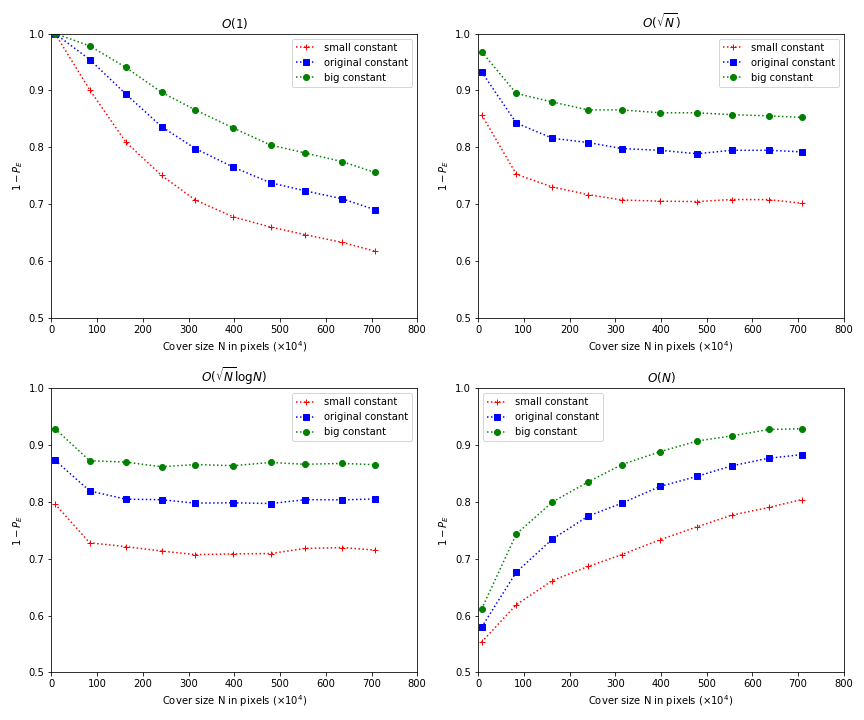
\includegraphics[width=\linewidth]{graph_29_03_2019.png}
    \end{center}

\end{itemize}

\section{08/03/19}

\begin{itemize}

  \item What I did:
    \begin{itemize}
      \item Computed two new sets of constants:
      \begin{center}
        \begin{tabular}{ c | c c c }
        & $-30\%$ & Original & $+30\%$ \\ \hline
        r1 & 49176.55272727272 & 70252.21818181817 & 91327.88363636362 \\
        r2 & 27.726656205965558 & 39.609508865665084 & 51.492361525364615 \\
        r3 & 1.2845357597929208 & 1.8350510854184585 & 2.385566411043996 \\
        r4 & 0.01563280510179924 & 0.022332578716856056 & 0.029032352331912873 \\
        \end{tabular}
      \end{center}
      
      \item Computed new payload sizes for the smaller constants:
      \begin{center}
        \begin{tabular}{ c c c | c c c c }
        Width & Height & Pixels & $O(1)$ & $O(\sqrt{n})$ & $O(\sqrt{n} \cdot \log n)$ & $O(n)$ \\ \hline
        3072 & 2304 & 7077888 & 49176 & 73764 & 77762 & 110647 \\
        2912 & 2184 & 6359808 & 49176 & 69922 & 73212 & 99421 \\
        2720 & 2040 & 5548800 & 49176 & 65312 & 67790 & 86743 \\
        2528 & 1896 & 4793088 & 49176 & 60702 & 62410 & 74929 \\
        2304 & 1728 & 3981312 & 49176 & 55323 & 56194 & 62239 \\
        2048 & 1536 & 3145728 & 49176 & 49176 & 49176 & 49176 \\
        1792 & 1344 & 2408448 & 49176 & 43029 & 42261 & 37650 \\
        1472 & 1104 & 1625088 & 49176 & 35345 & 33785 & 25404 \\
        1056 & 792 & 836352 & 49176 & 25356 & 23111 & 13074 \\
        320 & 240 & 76800 & 49176 & 7683 & 5777 & 1200 \\
        \end{tabular}
      \end{center}
      
      \item Computed new payload sizes for the larger constants:
      \begin{center}
        \begin{tabular}{ c c c | c c c c }
        Width & Height & Pixels & $O(1)$ & $O(\sqrt{n})$ & $O(\sqrt{n} \cdot \log n)$ & $O(n)$ \\ \hline
        3072 & 2304 & 7077888 & 91327 & 136991 & 144416 & 205487 \\
        2912 & 2184 & 6359808 & 91327 & 129856 & 135966 & 184640 \\
        2720 & 2040 & 5548800 & 91327 & 121294 & 125895 & 161094 \\
        2528 & 1896 & 4793088 & 91327 & 112732 & 115905 & 139154 \\
        2304 & 1728 & 3981312 & 91327 & 102743 & 104361 & 115586 \\
        2048 & 1536 & 3145728 & 91327 & 91327 & 91327 & 91327 \\
        1792 & 1344 & 2408448 & 91327 & 79911 & 78485 & 69922 \\
        1472 & 1104 & 1625088 & 91327 & 65641 & 62744 & 47180 \\
        1056 & 792 & 836352 & 91327 & 47090 & 42921 & 24281 \\
        320 & 240 & 76800 & N/A & 14269 & 10728 & 2229 \\
        \end{tabular}
      \end{center}

      \item Results (so far) of experiments using smaller and larger constants:
        \begin{center}
          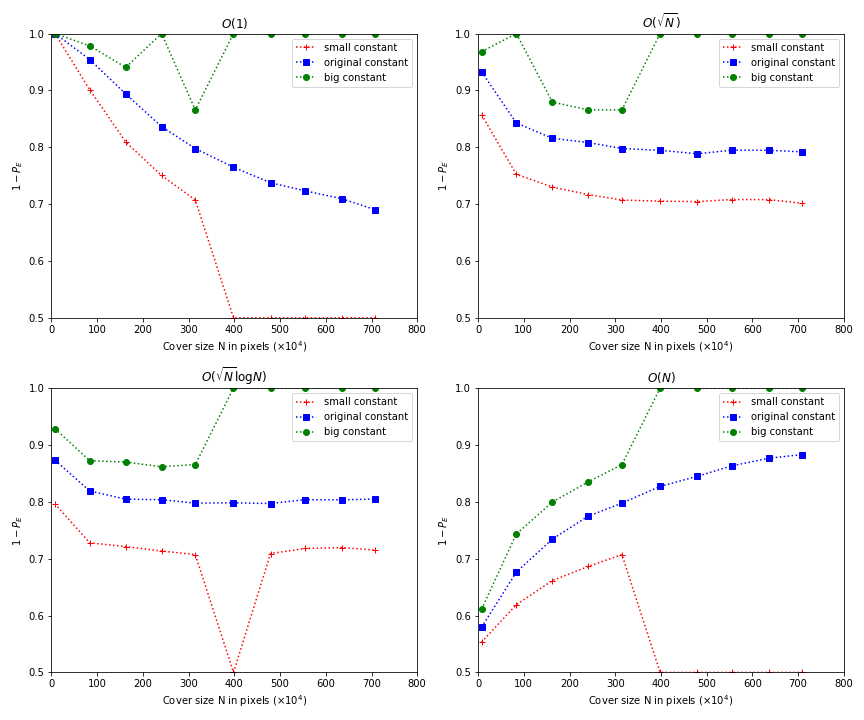
\includegraphics[width=\linewidth]{graph_07_03_2019.png}
        \end{center}

    \end{itemize}

  \item My next set of experiments will be on BOSSbase.

\end{itemize}


\section{01/03/19}

\begin{itemize}

  \item What I did:
    \begin{itemize}
      \item Finished all experiments and put together the results graph:
        \begin{center}
          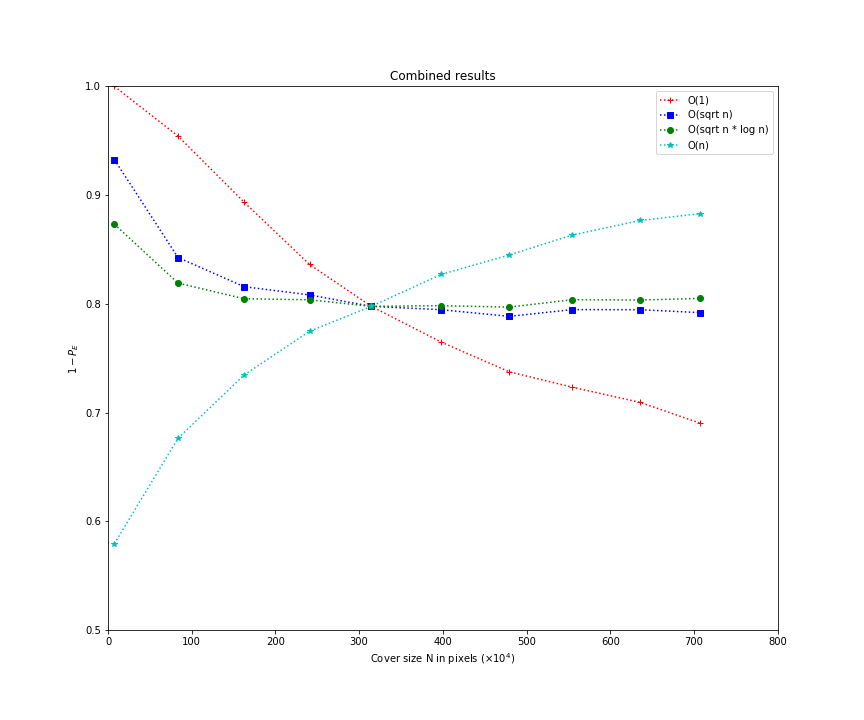
\includegraphics[width=\linewidth]{combined_graph_27_02_2019.png}
        \end{center}
      \item Miscellaneous:
        \begin{itemize}
          \item I parallelised the feature computation just like with embedding by looking at the last digit of the image numbers to spin up ten concurrent processes. Before, the feature files were being computed sequentially, which took 5-10 hours (depending on the image size). Now it takes less than 30 minutes.
          \item I tried using \texttt{at} for task scheduling, but realised that it means that I lose the timing information. This is because \texttt{at} either swallows the standard output/error or emails it to you, given the appropriate command line argument. But, there doesn't seem to be an appropriate email program installed and I don't know if it's worth it to use.
          \item A lot of timing information for the binary embedding was lost because somehow I (or my script) didn't specify/incorrectly specified a file for redirecting the standard output when running commands with \texttt{nohup}. It was all instead written to the default \texttt{nohup.out} file, which is now a big mess because many processes were writing to it concurrently. I made a note of all the tasks for which I have not timing information in my results tables at the end of this document.
          \item I made a copy of all the features into \texttt{/home} as a backup.
          \item I didn't end up applying to the BCS conference because of personal matters I had to deal with last week (deadline was Friday 22nd February) and because of uncertainty with what I was going to do over the break.
          \item I just booked my flights back to Canada and I am gone from 12th March to 4th April.
          \item I started adding papers to my bibliography. What format do I use? Which pieces of information are necessary (e.g. location, specific date as opposed to year)?
        \end{itemize}
      \item Next: do the same set of experiments but with two different constants - which ones?
    \end{itemize}

\item Now redo the experiment with two new sets of constants. These can be +/- 30\% of the existing ones. Should result in graphs with very similar shapes, just shifted slightly upwards and downwards, respectively.

\item I should also try training the classifier on all image sizes (e.g. a tenth of the images of each size) and then finding its error rate on images of each size.

\item It would be good to run these experiments on another images set. Dr. Ker will dig up the BOSSBase images and I can use these next.

\end{itemize}

\section{15/02/19}

\begin{itemize}

  \item What I did:
    \begin{itemize}
      \item Reran \texttt{calculate\_payload\_sizes.py} to get the right $O(\sqrt{n}\cdot\log{n})$ payload sizes (now $2048\times1536$ has the same payload size in all cases):
      \begin{center}
        \begin{tabular}{ c c c | c c c c }
        Width & Height & Pixels & $O(1)$ & $O(\sqrt{n})$ & $O(\sqrt{n} \cdot \log n)$ & $O(n)$ \\ \hline
        3072 & 2304 & 7077888 & 70252 & 105378 & 111089 & 158067 \\
        2912 & 2184 & 6359808 & 70252 & 99889 & 104589 & 142030 \\
        2720 & 2040 & 5548800 & 70252 & 93303 & 96843 & 123919 \\
        2528 & 1896 & 4793088 & 70252 & 86717 & 89158 & 107042 \\
        2304 & 1728 & 3981312 & 70252 & 79033 & 80278 & 88912 \\
        2048 & 1536 & 3145728 & 70252 & 70252 & 70252 & 70252 \\
        1792 & 1344 & 2408448 & 70252 & 61470 & 60373 & 53786 \\
        1472 & 1104 & 1625088 & 70252 & 50493 & 48264 & 36292 \\
        1056 & 792 & 836352 & 70252 & 36223 & 33016 & 18677 \\
        320 & 240 & 76800 & 70252 & 10976 & 8253 & 1715 \\
        \end{tabular}
      \end{center}
    \end{itemize}

\end{itemize}

\section{08/02/19}

\begin{itemize}

  \item What I did:
    \begin{itemize}
      \item Fixed problems with the binary embedding code.
        \begin{itemize}
          \item There was a problem with the exponential search for lambda getting stuck in an infinite loop. Then, I figured out that the floating point precision in the binary search for $\lambda$ was insufficient for finding a value of $\lambda$ such that the entropy sum is in the range $b \leq \lambda < b+1$, where $b$ is the number of payload bits. For $b = 70252$, it turned out that the entropy sum reached $70,253$ but could no longer be refined because the upper and lower bounds for $\lambda$ had reached the limits of the floating point precision.
        \end{itemize}
      \item Ran binary embedding on all image sizes for the $O(\sqrt{n})$ payloads (and all payload sizes for the $320\times240$ images)
        \begin{itemize}
          \item There were hangups in the middle of the embedding processes, so I killed all processes.
        \end{itemize}
      \item Noticed that the payload sizes computed for $O(\sqrt{n}\cdot\log{n})$ are wrong because the number of bits for the middle size is different from the the number of bits for the same size but other proportions. Probably a bug in the code.
    \end{itemize}

  \item The MinPE values for the processes that finished (only the ones for $320\times240$ images) look correct.
  
  \item There was indeed a bug in my \texttt{calculate\_payload\_sizes.py} script - I forgot to replace one of the calls to \texttt{log(x)} with \texttt{log(x,2)}, to use the right logarithm base.

\end{itemize}

\section{25/01/19}

\begin{itemize}

  \item What I did:
    \begin{itemize}
      \item Finished the graph template for the experiment results:
        \begin{center}
          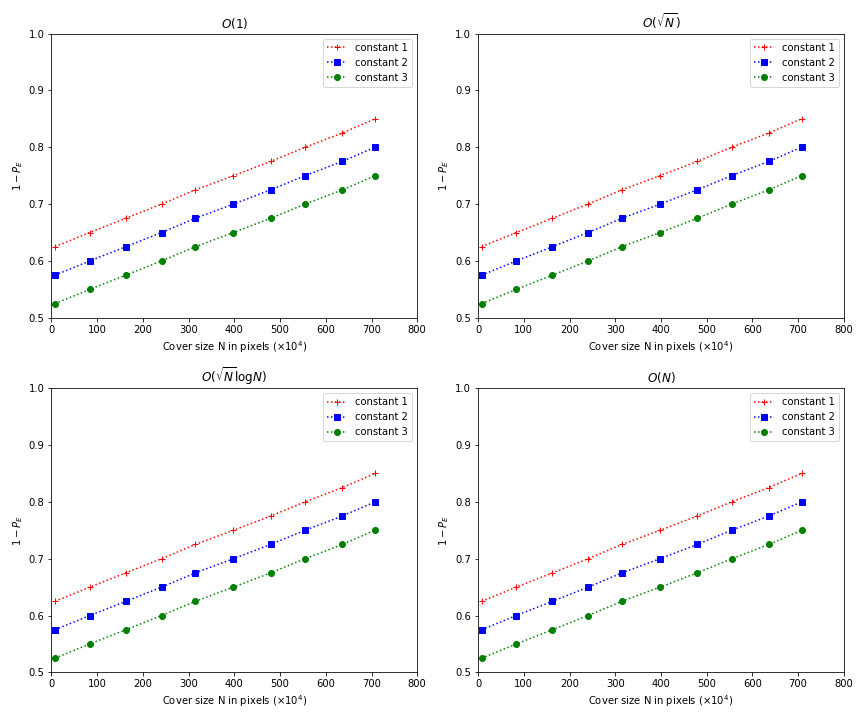
\includegraphics[width=0.7\linewidth]{graph_template.png}
        \end{center}
        \begin{itemize}
          \item If we decide to use only one proportionality constant for each payload size, then we will only have one plot per figure (rather than three like in the 2008 paper).
        \end{itemize}
    
      \item Finished writing the binary embedding code.
        \begin{itemize}
          \item Not quite working. Either throws an unknown error or behaves as if there are no images to process.
        \end{itemize}
    \end{itemize}

\end{itemize}

\section{11/01/19}

\begin{itemize}

  \item What I did:
    \begin{itemize}
      \item Finished running J-UNIWARD on all remaining images sizes.
      \item Picked values for $r_1, r_2, r_3, r_4$.
        \begin{itemize}
          \item The image size and $\alpha$ combination that produced a MinPE value closest to 20\% was $1056\times792$ with $\alpha=0.3$ (MinPE = 22\%).
          \item I ran \texttt{JPEG-UTILS} on all the $1056\times792$ images and found that the average number of non-zero coefficients was $120,746$.
          \item Since 0.3 bits per non-zero coefficient were embedded in each image, this means that an average of $0.3 \times 120,746 = 36,224$ bits were embedded per image.
          \item I chose $2048 \times 1536$ to be the "middle" image size. There are ten sizes, so it was either this or $2304 \times 1728$.
          \item I wrote a script \texttt{calculate\_payload\_sizes.py} that computes the number of bits that should be embedded for each image size for each proportion (i.e. $O(1)$, $O(\sqrt{n})$, $O(\sqrt{n} \cdot \log n)$, and $O(n)$, where $n$ is the number of pixels in each image).
          \item Compute the constant values computed as intermediate values by my script are:
            \begin{itemize}
              \item $r_1 = 70252.21818181817$
              \item $r_2 = 39.609508865665084$
              \item $r_3 = 2.64741910071112$
              \item $r_4 = 0.022332578716856056$
              \item For some reason, these values (and the values in the table below) differ when run on my computer versus on the server.
            \end{itemize}
          \item Using these constants, compute the number of bits to embed for each image size:
          \begin{center}
            \begin{tabular}{ c c c | c c c c }
            Width & Height & Pixels & $O(1)$ & $O(\sqrt{n})$ & $O(\sqrt{n} \cdot \log n)$ & $O(n)$ \\ \hline
            3072 & 2304 & 7077888 & 70252 & 105378 & 160268 & 158067 \\
            2912 & 2184 & 6359808 & 70252 & 99889 & 150891 & 142030 \\
            2720 & 2040 & 5548800 & 70252 & 93303 & 139714 & 123919 \\
            2528 & 1896 & 4793088 & 70252 & 86717 & 128628 & 107042 \\
            2304 & 1728 & 3981312 & 70252 & 79033 & 115816 & 88912 \\
            2048 & 1536 & 3145728 & 70252 & 70252 & 101352 & 70252 \\
            1792 & 1344 & 2408448 & 70252 & 61470 & 87100 & 53786 \\
            1472 & 1104 & 1625088 & 70252 & 50493 & 69631 & 36292 \\
            1056 & 792 & 836352 & 70252 & 36223 & 47632 & 18677 \\
            320 & 240 & 76800 & 70252 & 10976 & 11906 & 1715 \\
            \end{tabular}
          \end{center}
        \end{itemize}
    \end{itemize}

\item Later we can try training the classifier on all image sizes (maybe 10\% of the images of each size) and then run it against the images of each size. It can also be run against a set of images of multiple sizes.

\item Once we have the results, we can also try running all the experiments again on another set of images (from another actor).
  \begin{itemize}
    \item Actor 27 has 4890 images shot on an iPhone, but they are very small ($320 \times 480$).
    \item Actor 245 has 1524 images shot on an iPhone, of various different sizes.
    \item Actor 17 has a Sony camera with a good number of images and a nice camera.
    \item We could also use the original BossBase images (as opposed to the ones that have been shrunken down to $512 \times 512$). But a bit overused and artificial since they come from lots of different cameras.
  \end{itemize}

\item YFCC100m dataset

\end{itemize}

\section{03/12/18}

\begin{itemize}

\item What I did:
  \begin{itemize}
  \item Found a way to convert the features in the \texttt{imageXXXXX.fea} files into a format that the linear classifier can use.
    \begin{itemize}
    \item Wrote \texttt{combine\_feature\_files.py}, which creates a single file (e.g. \texttt{sizeX\_cover.fea}) with the features of all the images in a directory, one image per line. Each line is tab-separated and has the image name followed by the features (in row order).
    \item Wrote \texttt{txt\_to\_mat.m}, which takes a combined feature file and produces a \texttt{.mat} file that MATLAB can read to get the features in fields with names (and dimensions) that it expects.
    \end{itemize}

  \item Ran (ternary) J-UNIWARD embedding with $\alpha = 0.1$ on the six smallest image sizes.
    \begin{itemize}
    \item Realized that I wasn't reusing the J-UNIWARD costs I had previously computed, so I killed the processes that hadn't terminated yet (sizes  $1792 \times 1344, 2048 \times 1536, 2304 \times 1728$)
    \end{itemize}

  \item Created a modified J-UNIWARD that reads in the pre-computed costs from the \texttt{imageX.costs} files in the cover image directory.
    \begin{itemize}
    \item Started running this on the sizes that hadn't terminated without reusing costs.
    \item Sizes $1792 \times 1344, 2048 \times 1536, 2304 \times 1728$ haven't terminated yet although they've been running for several days.
    \end{itemize}

  \item Ran \texttt{compute\_features.py} on $J_{0.1}$ images (sizes $320 \times 240, 1056 \times 792, 1472 \times 1104$).
  
  \item Started working on modifying J-UNIWARD to do binary embedding.
  \end{itemize}

\end{itemize}


\section{21/11/18}

\begin{itemize}

\item What I did:
  \begin{itemize}
  \item Wrote \texttt{feature\_sanity\_check.py}, which adds up all the features for each image in a directory and outputs how many had the same sum (1346, a constant) and how many had zero sum (due to no features being generated).
    \begin{itemize}
    \item Ran it on all image sizes and found that the number of images for which the features weren't generated when I ran JRM on 10/11/18 increased as the image sizes increased.
    \end{itemize}

  \item Reran \texttt{compute\_features.py} on all images of all sizes.
     \begin{itemize}
     \item This time no images were skipped, which is good. However, the timing information was lost because for some reason the terminal output was not redirected to a file by \texttt{nohup}. This may have been caused by the fact that \texttt{nohup} was run by a Bash script for each file size and most likely I forgot the \texttt{\&} at the end of the line. All I know is that all processes finished after around 18-20 hours. This roughly matches the timing information from the original run on 10/11/18 when some images were skipped.
     \item I reran \texttt{feature\_sanity\_check.py} for all sizes. This confirmed that no images were skipped and that the sum of all features in each image of each size was 1346, as expected.
     \end{itemize}

  \item Changed \texttt{compute\_costs.py} so that Python's \texttt{multiprocessing} module is used for multithreading in order to spread out the cost computation over multiple processes to speed it up.
    \begin{itemize}
    \item I initially tried using Python's \texttt{threading} module, however creating multiple threads does not actually mean the computation is run in parallel due to Python's \href{https://docs.python.org/2/glossary.html\#term-global-interpreter-lock}{global interpreter lock (GIL)}.
    \item \texttt{multiprocessing}, on the other hand, avoids the limitations of the GIL and allows multiple processes (as opposed to threads) to be created and make use of multiple cores.
    \item \href{https://stackoverflow.com/a/3046201}{Here} is a good pro/con analysis of the two modules.
    \end{itemize}

  \item Ran \texttt{compute\_costs.py} on all images of all sizes.
    \begin{itemize}
    \item All cost files were generated, as expected.
    \item The terminal output is messy due to multiple processes printing concurrently. However, the total time is clearly visible on the last line of the terminal output.
    \end{itemize}

  \item TL;DR the costs and features of all cover images are all computed!
  
  \item Wrote my own program called \texttt{JPEG-UTILS}, which is based on the J-UNIWARD code and provides a number of checks and information about cover/stego images.
    \begin{itemize}
    \item Currently it provides two utilities:
      \begin{enumerate}
      \item Non-zero coefficient count: number of non-zero coefficients in a (cover) image
      \item Differing coefficients: number of coefficients that differ between cover/stego image pairs, broken down by the number that differ by +1, -1, or something else.      
      \end{enumerate}
    \end{itemize}

  \item Looked into how to implement my own binary embedding and it looks like there's no need to reinvent the wheel and the J-UNIWARD code can mostly be reused. Want to discuss.
  \end{itemize}

\item \textit{Should I rerun the feature computations just to get the timing information? It takes 18-20 hours.}
  \begin{itemize}
  \item I can, but it's not a priority now. I could do it later when I'm running the real experiments.
  \end{itemize}

\item The \texttt{float* pixel\_costs} in \texttt{cost\_model.cpp} of the J-UNIWARD code looks like it's initialized, filled, and then never used, but its ``initialization'' is actually C pointer arithmetic based on the address of the \texttt{float* costs} which is a field inherited from \texttt{base\_cost\_model.cpp}.

\item Equations for binary versus ternary embedding
  \begin{enumerate}
  \item Binary embedding
    \begin{itemize}
    \item This is the probability of changing coefficient $i$ by $\pm1$, where $c_i$ is the cost of changing coefficient $i$ (by $\pm1$) and $c_{\neg i} = 0$ is the cost of not changing it:
      \begin{equation*}
      \pi_i = \frac{1}{1+e^{\lambda c_i}} = \frac{1}{e^{\lambda c_{\neg i}}+e^{\lambda c_i}} = \frac{e^{-\lambda c_i}}{e^{-\lambda c_{\neg i}}+e^{-\lambda c_i}}
      \end{equation*}
    \item Entropy function for coefficient $i$:
      \begin{equation*}
      - \pi_i \log \pi_i - (1 - \pi_i) \log (1 - \pi_i)
      \end{equation*}
    \end{itemize}

  \item Ternary embedding
    \begin{itemize}
    \item This is the probability of changing coefficient $i$ by $+1$ (for example), where $c^0_i = 0$ is the cost of not changing coefficient $i$, $c^{+1}_i$ is the cost of changing it by $+1$, and $c^{-1}_i$ is the cost of changing it by $-1$:
    \begin{equation*}
    \pi^{+1}_i = \frac{e^{-\lambda c^{+1}_i}}{1+e^{-\lambda c^{+1}_i}+e^{-\lambda c^{-1}_i}} = \frac{e^{-\lambda c^{+1}_i}}{e^{-\lambda c^0_i}+e^{-\lambda c^{+1}_i}+e^{-\lambda c^{-1}_i}}
    \end{equation*}
      \begin{itemize}
      \item In practice, $c^{+1}_i = c^{-1}_i (= C \text{, say})$ for all $i$, meaning that the costs of adding one versus substracting one are the same, so:
      \begin{equation*}
      \pi^{+1}_i =\pi^{-1}_i =  \frac{e^{-\lambda C}}{1+2 \cdot e^{-\lambda C}}
      \end{equation*}
      \end{itemize}
    \item Entropy function for coefficient $i$:
      \begin{equation*}
      - \pi^{+1}_i \log \pi^{+1}_i - \pi^{-1}_i \log \pi^{-1}_i - \pi^0_i \log \pi^0_i
      \end{equation*}
    \end{itemize}
  \end{enumerate}

\item \textit{Can I reuse the structure of the J-UNIWARD code to implement binary embedding?}
  \begin{itemize}
  \item Yes, but I need to be careful to make sure things are read in the right order and all methods whose implementations are specifically for ternary embedding are adapted to be for binary embedding.
  \item Specifically, the entropy function and probability computation need to be changed to use the equations described in the point above.
  \item I also need to adapt it so that it takes a number of bits as an argument instead of the number of bits per non-zero coefficient.
  \end{itemize}

\item The \href{http://dde.binghamton.edu/kodovsky/pdf/SPIE2012_Kodovsky_Steganalysis_of_JPEG_Images_Using_Rich_Models_paper.pdf}{JRM paper} describes how JRM produces 22,510 features. These are actually made up of two sets of 11,255 features, one for the image itself and one for the same image, but with 4-pixel strips cropped off all sides (``Cartesian calibration'').
  \begin{itemize}
  \item The reason the features all add up to the same constant for each image, regardless of size, is that the features are normalized so that they sum to 1. The way JRM computes the features is based on ``submodels'' and all images have the same number of submodels (672) regardless of size.
  \item The features within each submodel (something like this) are normalized, so summing all the features of both halves (from the two versions of the image), makes a total sum of $672\cdot1 + 672\cdot1 = 1346$, which is what we get when running \texttt{feature\_sanity\_check.py}.
  \end{itemize}

\item When I run J-UNIWARD for the pre-experiments, I should actually use 0.1 instead of 0.4 as previously discussed.
  \begin{itemize}
  \item For BOSSbase, where all images are $512 \times 512$, $\alpha = 0.2$ produced a ``good'' classification error rate. However, those images are about $\frac{1}{4}$ of a megapixel whereas the middle size images in our dataset are about $3$ megapixels.
  \end{itemize}

\item Step-by-step explanation of how we'll choose constants $r_1, ... , r_4$ in order to compute the number of bits of payload to embed. \underline{Goal}: pick them such that $r_1 = r_2 \cdot \sqrt{n_{mid}} = r_3 \cdot \sqrt{n_{mid}} \cdot \log n_{mid} = r_4 \cdot n_{mid}$, where $n_{mid}$ is the number of pixels in the ``middle'' image size.
  \begin{enumerate}
  \item Run J-UNIWARD with $\alpha = 0.1$ on some of the image sizes (among the smaller half of the sizes).
  \item Compute the features of these stego images and then train and run the classifier on these cover-stego image pairs.
  \item Record the classifier's error rate (call it $P_e$) for each image size.
  \item We want to find an image size where $P_e \approx 20\%$. Using \texttt{JPEG-UTILS}, see how many non-zero coefficients there were on average and then use this and $\alpha = 0.1$ to compute the average number of bits that were embedded (well, simulated).
  \item Assuming the square root law holds, pro-rate this to compute the number of bits that should be embedded in the middle image size. Call this $m^{\ast}_{mid}$.
  \item Knowing $m^{\ast}_{mid}$ and $n_{mid}$, compute $r_1, ... , r_4$ so that:
    \begin{align*}
    m^{\ast}_{mid} &= r_1 \\
    m^{\ast}_{mid} &= r_2 \cdot \sqrt{n_{mid}} \\
    m^{\ast}_{mid} &= r_3 \cdot \sqrt{n_{mid}} \cdot \log n_{mid} \\
    m^{\ast}_{mid} &= r_4 \cdot n_{mid}
    \end{align*}
  \end{enumerate}

\item 95\% confidence interval formula (where $P$ is the error rate and $n$ is the sample size):
  \begin{equation*}
  \pm 1.96 \cdot \sqrt{\frac{P \cdot (1-P)}{n}}
  \end{equation*}

\item We don't need to worry about splitting the data into training, validation, and testing sets. We can let the classifier handle it using its default behaviour. We're not too concerned about doing ``perfect'' machine learning since we can't get many significant figures in our rates in a statistically significant way given that we only have 10,000 images.

\end{itemize}


\section{14/11/18}

\begin{itemize}

\item What I did:
  \begin{itemize}
  \item Ran the hacked J-UNIWARD to compute the costs of all the images of all sizes.
    \begin{itemize}
    \item It computed the costs of all the $320 \times 240$ images after about 2 hours, but the processes computing the costs for the other sizes either terminated in the middle of their execution (before finishing all images), or did not terminate at all (in the case of $2912 \times 2184$ and $2720 \times 2040$) althought they were not making any progress.
    \end{itemize}

  \item Wrote \texttt{compute\_features.py}, which runs JRM on all the JPEGs in a directory and saves the results to a \texttt{.fea} file.
  
  \item Ran \texttt{compute\_features.py} on all images of all sizes.
    \begin{itemize}
    \item All ten processes terminated and processed all images.
    \item The slowest one took 1h22m and the longest one took 20h4m.
    \item However, some of the \texttt{.fea} files generated were empty and I don't know why.
    \end{itemize}

  \item Was sick the last week, so didn't get much else done.
  \end{itemize}

\item The timing of me running J-UNIWARD and JRM (in parallel) coincided with some issues on the server with regard to memory.
  \begin{itemize}
  \item It ended up being restarted, so I should just rerun everything.
  \item Apparently, JRM does sometimes silently fail. However, when I reran it on some of the images whose features were not computed, it worked which was odd.
  \end{itemize}

\item It's possible that there was an issue with the simultaneous cost and feature computations because the \texttt{compute\_features.py} iterated through all files in the directory while more files were being generated both by itself and by J-UNIWARD.
  \begin{itemize}
  \item When rerunning the computations, I'll modify my script to iterate from 1 to 13349 to ``create'' the image names itself (and check that they actually exist, since not all 13349 images were used), which will avoid any issues with simultaneous directory iteration and file generation.
  \end{itemize}

\item The sums of the features of each image should be a constant, so it would be a good idea to do a sanity check to ensure that this is indeed the case.

\item To make the cost and feature computations go faster, it would be a good idea to spin off multiple threads (in Python).
  \begin{itemize}
  \item For instance, I could spin off 10 threads and make thread 1 handle images with number 1 (mod 10).
  \end{itemize}

\item Before running experiments, we need to choose constants $r_1, ... , r_4$ in order to compute the number of bits of payload to embed.
  \begin{itemize}
  \item Amounts: $r_1, r_2 \cdot \sqrt{n}, r_3 \cdot \sqrt{n} \cdot \log n, r_4 \cdot n$ for each \# of pixels $n$.
  \item To choose $r_1, ... , r_4$, we do the following:
    \begin{enumerate}
    \item Run J-UNIWARD with 0.4 bits per non-zero coefficient for all (or every other) image size.
    \item Write and run a script that counts the number of coefficients that differ between the cover and stego images.
    \item From those counts, compute the number of bits that were embedded for each size.
    \item Compute the features of the stego images.
    \item Train the classifier with the features of the cover and stego images.
    \item Run the classifier to determine detectability for each image size.
    \item ...? CLARIFY
    \end{enumerate}
  \item We'll choose $r_1, ... , r_4$ such that the ``middle'' image size is in the ``middle'' among image sizes in terms of detectability. CLARIFY
  \item Something about number of non-zero coefficients...
  \end{itemize}

\end{itemize}


\section{07/11/18}

\begin{itemize}

\item What I did:
  \begin{itemize}
  \item Created the file structure on the server.
    \begin{itemize}
    \item Each \texttt{actor00003/sizeXXXX/} directory has one subdirectory called \texttt{cover}.
    \item We need to decide/calculate how many bits of payload to embed for each size before creating subdirectories for all the different payload sizes.
    \end{itemize}

  \item Changed \texttt{initial\_curation.py} so that constants in the file are instead passed in as command-line arguments.
    \begin{itemize}
    \item Reran it and it was almost twice as fast (11 vs 19 minutes), though the speedup is probably not related to this change.
    \end{itemize}

  \item Finished \texttt{compute\_probabilities.py}. It finds a $\lambda$ such that:
    \begin{equation*}
    \sum\limits_{i=1}^N H_2(\pi_i) \in [m, m+1)\text{, where $m$ is the payload size to simulate}
    \end{equation*}

  \item Wrote \texttt{crop.py} and ran it for the other nine image sizes.
    \begin{itemize}
    \item It crops $8\times8$ blocks evenly from the top/bottom and right/left.
    \item The process is documented in Section \ref{subsec:cropping}.
    \end{itemize}

  \item Refactored the J-UNIWARD code (C++ source files) for readability and uploaded them to my GitHub repository in the \texttt{j-uniward} directory.
    \begin{itemize}
    \item Created a version that integrates Dr. Ker's hack to save the costs to a file (in ASCII) without doing the actual embedding.
    \item 99\% sure the costs are output in row order, which would be the intuitive way to implement it.
  \end{itemize}

  \item Started working on \texttt{compute\_costs.py}, which runs the hacked J-UNIWARD on all images in a directory.
  \end{itemize}

\item Computing the costs for all the images of all sizes
  \begin{itemize}
  \item On one core, it will take:
    \begin{equation*}
    50s \times 10000 \times (1 + 0.9 + ... + 0.1) \approx 763 \text{ hours} \approx 32 \text{ days}
    \end{equation*}
  \item I can use 8-10 of the server's 40 cores.
  \item I'll run the script using \texttt{nohup} once per directory and obviously the process will finish faster for the smaller images, so I can start on the next task (feature computation) with those that finish first.
  \end{itemize}

\item Once the costs are computed, the next task is computing the features using JRM.

\item Then, I'll start by using J-UNIWARD with 0.4 bits per non-zero coefficient. I then need to compute the features of the stego objects. Once this is done, I can train the classifier with the features of all the cover and stego objects.
  \begin{itemize}
  \item The original plan was to use the \href{http://dde.binghamton.edu/download/ensemble/}{ensemble classifier}.
  \item We will instead use a \href{http://dde.binghamton.edu/download/LCLSMR/}{low-complexity linear classifier}, which achieves similar performance but has a lower computational complexity.
  \end{itemize}

\item When training the classifier, it's important to keep the cover/stego objects pairs together (i.e. not put the cover in the training set and the stego in the testing test for cross-validation).
  \begin{itemize}
  \item This is important because it ensures the classfier learns the correct boundary.
  \end{itemize}

\item The binary embedding I'll write will take the number of bits to embed as input.
  \begin{itemize}
  \item We will compute the specific number of bits to run the embedding with by manually computing $r \cdot \sqrt{n}$ and $r \cdot \sqrt{n} \cdot \log n$, where $n$ is the total number of pixels in each image and $r$ is some constant we'll pick.
  \item We'll pick $r$ such that it makes the detectability of the ``middle'' image size the median among the detectabilities of all the sizes, where ``detectability'' refers to the classifier's accuracy.
  \end{itemize}

\item When the classifier training function asks for the costs ``row-by-row'', they mean it should be a big matrix where the first half of the rows are the costs of the cover images, in order, and the second half are the costs of the stego images, in the same order.

\end{itemize}


\section{31/10/18}

\begin{itemize}

\item What I did:
  \begin{itemize}
  \item Put together this document
  \item Organized all documents and scripts in my (private) GitHub repository
  \item Fixed \texttt{initial\_curation.py} (the problem is documented in Section \ref{sec:lessons-learned}) and I successfully ran it on the server
    \begin{itemize}
    \item Original images: \texttt{/array/vlasov/actor00003/original}
    \item All $3072\times2304$, grayscale, landscape images are in a new directory \texttt{/array/vlasov/actor00003/size3072}
    \end{itemize}
  \item Learned how to use \texttt{pyplot}, plotted $H_2$ as an exercise
  \item Computed the image sizes we'll use (the process and results are described in Section \ref{subsec:image-sizes})
    \begin{itemize}
    \item The method discussed on 24/10/18 doesn't work. It does produce equally sized intervals (in terms of the difference in the total number of pixels between consecutive sizes), but only between $320\times240$ and the ninth-largest size since this interval is only around $70,000$. The ninth-largest size would be $960\times720$, which is clearly much smaller than $3072\times2304$.
    \item In order to get sizes linearly distributed in terms of the total number of pixels, the interval needs to be closer to $700,000$ pixels.
    \end{itemize}
  \item Started working on \texttt{compute\_probabilities.py}
  \end{itemize}

\item \textit{Is the value of $\lambda$ bounded? How should the binary search (in the context of PLS) work?}
  \begin{itemize}
  \item $\lambda = 0$ corresponds to maximum entropy (aka. maximum payload) because then $\pi_i = \frac{1}{1+e^{\lambda c_i}} = \frac{1}{2}$

  \item As $\lambda \rightarrow \infty$, $\pi_i \rightarrow 0$

  \item The order of magnitude of $\lambda$ depends on the order of magnitude of the costs.

  \item The binary search will have two stages:
    \begin{enumerate}
    \item Exponential search to find an upper bound on $\lambda$. This will involve trying exponentially large values such as $0, 1, 10, 100, ...$ until a value is found such that $\sum\limits_{i=1}^N H_2(\pi_i) < M$
    \item Suppose the first value where this inequality holds is $\lambda = 10^n$. We now do a binary search for $\lambda$ with a lower bound of $10^{n-1}$ and an upper bound of $10^n$ and we want to find a value such that $\sum\limits_{i=1}^N H_2(\pi_i) \in [m, m+1)$, where $m$ is the number of payload bits.
    \end{enumerate}
  \end{itemize}
  
\item In Dr. Ker's paper ``On the Relationship Between Embedding Costs and Steganographic Capacity'' from June 2018, he writes about how if the detector knows the costs $c_1, c_2, ... c_N$, then the objective that should be minimized is $\sum\limits_{i=1}^N c_i \pi_i^2$, which is the same as the objective in PLS except with the $\pi_i$ terms squared.
  \begin{itemize}
  \item This is a possible project extension.

  \item The tricky part is computing the probabilities since the optimal solution is no longer $\pi_i = \frac{1}{1+e^{\lambda c_i}}$. Instead, it's $\frac{\pi_i}{H_{2}'(\pi_i)} = \lambda c_i$.

  \item The probabilities can be computed by running Newton-Raphson several times (Dr. Ker did it 8 times)

  \item I don't need to tackle this now, but it's worth keeping in mind.
  \end{itemize}

\item When I use Dr. Ker's J-UNIWARD hack, I need to make sure that I work out the order in which the costs are written to the file.
  \begin{itemize}
  \item It's hard to tell just by looking at the costs whether or not they're in the right order. If I'm wrong, I'll probably find out since the embedding will be very detectable.
  \item It's very likely that the $8\times8$ blocks are analyzed from left to right, top to bottom. However, within each block the costs could be left to right, top to bottom \textbf{or} in the zigzag order used to store the quantized coefficients. I need to check this.
  \end{itemize}

\item Once I compute the probabilities, it might be a good idea to use Python's \texttt{random.seed(..)} method (with the image number as the seed) in order to do the embedding. It can be used to determine whether or not to change each coefficient and so I'll always get the same embedding with the same cover, modulo rounding.

\item Dr. Ker has a faster version of JRM for feature extraction.

\item Tips:
  \begin{itemize}
  \item After embedding, open the stego image to make sure nothing got messed up (e.g. due to the order of the costs or coefficients).

  \item It would be a good idea to write some scripts to check things like:
    \begin{itemize}
    \item The number of coefficients that differ between the cover and stego images is $\approx \sum\limits_{i=1}^N \pi_i$
    \item Coefficients that differ between the cover and stego images only differ by $\pm1$
    \end{itemize}

  \item Test things out on small images (e.g. $64\times64$) to save time in case there are bugs.
  \end{itemize}

\end{itemize}


\section{24/10/18}

\begin{itemize}

\item What I did:
  \begin{itemize}
  \item Read Chapter 3 of the Advanced Security notes on steganography
  \item Wrote a script (\texttt{initial\_curation.py}) to find all the largest images in the \texttt{actor00003} directory and then make them all grayscale and landscape (described in Section \ref{subsec:initial-image-selection})
    \begin{itemize}
    \item Wasn't quite working due to ``\texttt{Empty input file}'' error when performing multiple \texttt{jpegtran} operations
    \end{itemize}
  \end{itemize}

\item Action plan:
  \begin{enumerate}

  \item Calculate image sizes
    \begin{itemize}
    \item Preserve the 4:3 aspect ratio, not because we have to but because we can and it means we can keep things as similar as possible

    \item The largest image size we'll use is $3072\times2304$ since that's the size of the largest \texttt{actor00003} images.

    \item The smallest size will be $320\times240$ since that's a relatively common image size (and it has a 4:3 aspect ratio)

    \item The short-edge dimensions will be computed by hand by calculating $240x$ (where $x=\sqrt{1}, \sqrt{2},...,\sqrt{10}$) and then rounding to the nearest multiple of 24. Then the long-edge dimensions are calculated such that the 4:3 ratio is maintained.
    \end{itemize}

  \item Create the directory structure on the server in \texttt{/array/vlasov/}
    \begin{itemize}
    \item Keep a copy of all the original images in \texttt{actor00003/original}

    \item Create one directory per image size, called \texttt{size3072} (for instance)

    \item For each size, create two subdirectories:
      \begin{enumerate}
      \item One for the unaltered images, called \texttt{cover}
      \item One per number of payload bits, called \texttt{stego-1234bits}
      \end{enumerate}

    \item Each \texttt{cover} subdirectory will have three files per cover image:
      \begin{enumerate}
      \item \texttt{image12345.jpg}: the unaltered image
      \item \texttt{image12345.costs}: the costs computed by J-UNIWARD
      \item \texttt{image12345.fea}: the features computed by JRM
      \end{enumerate}

    \item Each \texttt{stego-1234bits} subdirectory will have one file per stego image:
      \begin{enumerate}
      \item \texttt{image12345.jpg}: the stego image, which is the cover image \texttt{sizeXXXX/cover/image12345.jpg} with a 1234-bit message embedded in it
      \end{enumerate}
    \end{itemize}

  \item Crop the $3072\times2304$ cover images to the sizes calculated in task 1. Do this by cropping $8\times8$ pixel blocks evenly from the top/bottom and right/left.

  \item Generate the costs (using Dr. Ker's slighty modified J-UNIWARD code) and features (using JRM) for all the cover images of all the different sizes.
  \begin{itemize}
  \item JRM produces 22510 real numbers (the features)
  \item Up to me how to store them, but ASCII is probably the most portable
  \end{itemize}

  \item Use J-UNIWARD to embed 0.4 bits per non-zero AC coefficient in some of the covers.

  \item Write a function that takes the number of payload bits as input and computes the probabilities with which each coefficient changes during (binary) embedding.
    \begin{itemize}
    \item Goal: given the costs $c_1, c_2, ... c_N$ (where N is the total number of coefficients) of changing each coefficient (by adding or subtracting one), compute the probabilities $\pi_1, \pi_2, ..., \pi_N$ of making each of these changes

    \item Size of the payload: $\sum\limits_{i=1}^N H_2(\pi_i)$
      \begin{itemize}
      \item $H_2$ is the ``entropy'' and is defined as:
        \begin{equation*}
        H_2(x) = -x \cdot \log_2 x - (1-x) \cdot \log_2 (1-x)
        \end{equation*}

      \item Graph of $H_2$:
        \begin{center}
          \includegraphics[width=0.7\linewidth]{h2_plot.png}
        \end{center}
      \end{itemize}

    \item Average total cost: $\sum\limits_{i=1}^N c_i \pi_i$

    \item Two (equivalent) optimization problems for computing the payload size:
      \begin{enumerate}
      \item Distortion-limited sender (DLS)
        \begin{equation*}
        \text{Maximize } \sum\limits_{i=1}^N H_2(\pi_i) \text{ such that } \sum\limits_{i=1}^N c_i \pi_i \leq C
        \end{equation*}

      \item Payload-limited sender (PLS)
        \begin{equation*}
        \text{Minimize } \sum\limits_{i=1}^N c_i \pi_i \text{ such that } \sum\limits_{i=1}^N H_2(\pi_i) \geq M
        \end{equation*}
      \end{enumerate}

    \item For some fixed $\lambda$, we can compute the probabilities:
      \begin{equation*}
      \pi_i = \frac{1}{1+e^{\lambda c_i}}
      \end{equation*}

    \item We'll use PLS, where M is the payload size.
      \begin{itemize}
      \item The optimal solution is when $\sum\limits_{i=1}^N H_2(\pi_i) = M$
      \item $\sum\limits_{i=1}^N H_2(\pi_i)$ is actually monotonically decreasing, so we can find a value of $\lambda$ such that $\sum\limits_{i=1}^N H_2(\pi_i) = M$ for any M we choose. Then, we can compute the probabilities $\pi_1, \pi_2, ..., \pi_N$ using this value of $\lambda$.
      \item The end goal is to do the embedding ourselves by modifying each coefficient with these probabilities.
      \end{itemize}
    \end{itemize}

  \end{enumerate}

\item \textit{Is 80 a standard JPEG quality factor (QF)?} In the massive image database released by Flickr, the most common QFs were 100, the QF used by iPhones, and 80. So, we're using 80 because that gives us a greater selection of images.

\end{itemize}


\section{17/10/18}

\begin{itemize}

\item What I did:
  \begin{itemize}
  \item Read Chapters 1 and 2 of the Advanced Security notes on steganography
  \item Read the 2008 paper ``The Square Root Law of Steganographic Capacity''
  \end{itemize}

\item Discussed questions I had about Chapter 1 (Steganography) and Chapter 2 (Steganalysis) of the Advanced Security notes and about the 2008 paper.
  \begin{itemize}

  \item \textit{What is downsampling?} Shrinking

  \item \textit{When you take a pictures on your phone, what happens?} Captures raw image, immediately compresses it as a JPEG, and discards the raw image

  \item \textit{What determines a cover's ``source''?} Primarily the camera. The camera's ISO setting, in particular, is very important. The subject of the photos don't make much of a difference.

  \item \textit{In JPEG compression, don't you lose some information when dividing the image into $8\times8$ pixel blocks?} No, the DCT is linear (i.e. 1-to-1 mapping from $8\times8$ blocks to coefficients)

  \item \textit{Is a JPEG decompressed every time you view it on a computer?} Yes

  \item \textit{When LSBR is used on RGB images, which bit(s) are changed?} Good question - it depends, but usually the LSBs of all three components (in sync)

  \end{itemize}

\item After embedding a payload, the original cover is destroyed. Otherwise, two nearly identical images would be floating around and Alice could easily be outed if someone got their hands on both versions.

\end{itemize}


\section{03/10/18}

\begin{itemize}

\item What I did: N/A

\item Discussed software to be used for embedding (J-UNIWARD), feature extraction (JRM), and detection (ensemble of linear classifiers)
  \begin{itemize}
  \item All the software is \href{http://dde.binghamton.edu/download/stego_algorithms/}{here}
  \end{itemize}

\item Server's IP: 163.1.88.150

\item Amounts of payload to embed: $O(1)$, $O(\sqrt{n})$, $O(\sqrt{n} \log n)$, $O(n)$

\item $m \sim \frac{\sqrt{DC}}{2} \log \frac{C}{D}$

\item TIME EVERYTHING

\item I will test new embedding and new detecting methods and I could also try old embedding and new detecting methods

\item Total amount of space needed (assuming around 10,000 images are used):
  \begin{itemize}
  \item Images: $2MB \times 10000 \times 9 \approx 180GB$
  \item Costs: $8B \times 5M \times 10000 \approx 400 GB$
  \item Features: $170KB \times 10000 \times 9 \approx 17GB$
  \end{itemize}

\end{itemize}


%-----------------------
\chapter{Notes to Self}

\section{Useful Commands}

\begin{itemize}

\item Run a command in the background so that you can keep using the terminal or close it
  \begin{itemize}
  \item \texttt{nohup python script.py \&> script\_output.out \&}
  \end{itemize}

\item Check on processes that are running
  \begin{itemize}
  \item \texttt{ps aux | grep vlasov}
  \end{itemize}

\item See what processes are currently running, how many resources they're using, etc.
  \begin{itemize}
  \item \texttt{htop}
  \end{itemize}

\item View information on how much RAM is used, available, etc.
  \begin{itemize}
  \item \texttt{free}
  \end{itemize}

\item Compile MATLAB code
  \begin{itemize}
  \item \texttt{mcc -m [-v] abc\_xyz.m}
  \end{itemize}

\item Run script generated by \texttt{mcc}
  \begin{itemize}
  \item \texttt{./run\_abc\_xyz.sh /usr/local/matlab-r2014a/}
  \end{itemize}

\end{itemize}


\section{Experiment Pipeline}
\begin{enumerate}
  \item Pre-processing: \texttt{actor3\_preprocessing.py} or \texttt{bossbase\_preprocessing.py}
  \item Cropping: \texttt{crop.py}
  \item Costs: \texttt{compute\_costs.py}, \texttt{J-UNIWARD-COSTS}
  \item Features: \texttt{do\_fea\_partitioned.sh}, \texttt{compute\_features.py}, \texttt{jrm}
  \item Embedding:
    \begin{itemize}
      \item Ternary J-UNIWARD: \texttt{J-UNIWARD-EMBED-WITH-COSTS}
      \item Binary J-UNIWARD: \texttt{BINARY-EMBED}
    \end{itemize}
  \item Feature matrix: \texttt{combine\_feature\_files.py} then \texttt{run\_txt\_to\_mat.sh}
  \item Linear classifier: \texttt{run\_juniward\_test.sh}
\end{enumerate}

\section{Lessons Learned}
\label{sec:lessons-learned}

\begin{itemize}

\item The input and output file to \texttt{jpegtran} can't be the same, otherwise you get an ``\texttt{Empty input file}'' error.

\item If it looks like directories on the server have disappeared, turn off f.lux or change the colour settings in \texttt{.bashrc}.

\item Beware that in Python versions earlier than 2.3, the \texttt{log} function computes the natural logarithm. In version 2.3, an optional \texttt{base} argument was added in order to specify the base of the logarithm. So, if you execute \texttt{log(64,2)} with a Python version earlier than 2.3, the second argument is ignored and you get the natural logarithm of 64.

\item If I use \texttt{at} to schedule tasks, I will not have access to the standard output because it tries to email it to me, which fails because there is no mail transfer agent installed.

\item Back up features (\texttt{.mat} files) to \texttt{/home} because it is backed up whereas \texttt{/array} is not. Nothing happened yet, but just in case. Last backup was 27/02/19.

\end{itemize}


%-----------------------
\chapter{Actor3 Experiment Results}
\label{sec:actor3-results}

\section{Cover Images}
\subsection{Pre-Processing}
\begin{itemize}
    \item 01/11/18: $655.185225964s \approx$ 10m55s
\end{itemize}

\subsection{Cropping}
\begin{itemize}
  \item 01/11/18:
  \begin{center}
  \begin{tabular}{ c c | c c }
  W & H & Seconds & Approx. Time\\ \hline
  2912 & 2184 & 689.414359808 & 11m29s \\
  2720 & 2040 & 662.552460909 & 11m02s \\
  2528 & 1896 & 662.54279089 & 11m02s \\
  2304 & 1728 & 632.872202158 & 10m32s \\
  2048 & 1536 & 605.926501989 & 10m05s \\
  1792 & 1344 & 555.097690105 & 9m15s \\
  1472 & 1104 & 511.460752964 & 8m31s \\
  1056 & 792 & 438.49830699 & 7m18s \\
  320 & 240 & 359.436480045 & 5m59s \\
  \end{tabular}
  \end{center}
\end{itemize}

\subsection{Costs}
\begin{itemize}
  \item 17/11/18:
  \begin{center}
  \begin{tabular}{ c c | c c }
  Width & Height & Seconds & Approx. Time \\ \hline
  3072 & 2304 & 202775.362686 & 2d 8h 19m \\
  2912 & 2184 & 194673.499774 & 2d 6h 4m \\
  2720 & 2040 & 183598.260891 & 2d 2h 59m \\
  2528 & 1896 & 172031.831308 & 1d 23h 47m \\
  2304 & 1728 & 152188.728338 & 1d 18h 16m \\
  2048 & 1536 & 129785.996801 & 1d 12h 3m \\
  1792 & 1344 & 104988.846009 & 1d 5h 9m \\
  1472 & 1104 & 74601.1954741 & 10h 43m \\
  1056 & 792 & 39340.753726 & 10h 55m \\
  320 & 240 & 3767.95246005 & 1h 2m \\
  \end{tabular}
  \end{center}
\end{itemize}

\subsection{Features}
\begin{itemize}
\item 10/11/18:
  \begin{center}
  \begin{tabular}{ c c | c c }
  Width & Height & Seconds & Approx. Time \\ \hline
  3072 & 2304 & 72,282.4331231 & 20h4m \\
  2912 & 2184 & 63,869.6948001 & 17h44m \\
  2720 & 2040 & 54,000.526902 & 15h0m \\
  2528 & 1896 & 40,194.252851 & 11h9m \\
  2304 & 1728 & 32,157.8610289 & 8h55m \\
  2048 & 1536 & 30,295.748122 & 8h24m \\
  1792 & 1344 & 18,653.2866731 & 5h10m \\
  1472 & 1104 & 14,390.2565191 & 3h59m \\
  1056 & 792 & 8,721.86998391 & 2h25m \\
  320 & 240 & 6,430.11 & 1h22m \\
  \end{tabular}
  \end{center}
  \begin{itemize}
  \item On 15/11/18, I checked the sums of the features to ensure that they all add up to the same constant. This constant turns out to be 1346 for each image's features, regardless of size.
  \item However, it turns out that several hundred images' features were not computed.
  \end{itemize}
\item 17/11/18: Unfortunately the timing information wasn't logged, but as a general idea, all processes finished after around 18-20 hours.
\end{itemize}

\subsection{Feature Matrix}
\begin{itemize}
\item 02/12/18:
  \begin{itemize}
  \item Combine feature files: \textit{Timing information lost}
  \item Convert to MATLAB matrix (no timing information)
  \end{itemize}
\end{itemize}

\section{Ternary Embedding (\texorpdfstring{$\alpha=0.1$}{alpha})}
\subsection{Embedding}
  \begin{center}
  \begin{tabular}{ r r | r r r }
  Width & Height & Seconds & Time & Date Finished \\ \hline
  2304 & 1728 & -- & -- & 13/12/18 \\
  2048 & 1536 & -- & -- & 12/12/18 \\
  1792 & 1344 & -- & -- & 12/12/18 \\
  1472 & 1104 & 316072 & 3d15h & 02/11/18 \\
  1056 & 792 & 35545 & 9h52m & 29/11/18 \\
  320 & 240 & 3192.98 & 53m & 29/11/18 \\
  \end{tabular}
  \end{center}

\subsection{Features}
  \begin{center}
  \begin{tabular}{ r r | r r r }
  Width & Height & Seconds & Time & Date \\ \hline
  2304 & 1728 & 13062.3725212 & 3h37m & 13/12/18 \\
  2048 & 1536 & 12428.002079 & 3h27m & 13/12/18 \\
  1792 & 1344 & 8581.41911697 & 2h23m & 12/12/18 \\
  1472 & 1104 & 8461.04521799 & 2h21m & 02/12/18 \\
  1056 & 792 & 5645.03076911 & 1h34m & 02/12/18 \\
  320 & 240 & 735.175777912 & 12m & 29/11/18 \\
  \end{tabular}
  \end{center}

\subsection{Feature Matrix}
\begin{itemize}
  \item Combine feature files:
  \begin{center}
  \begin{tabular}{ r r | r r r }
  Width & Height & Seconds & Time & Date \\ \hline
  2304 & 1728 & 39.6396141052 & 39s & 13/12/18 \\
  2048 & 1536 & 40.74949193 & 40s & 13/12/18 \\
  1792 & 1344 & 80.3196239471 & 1m20s & 13/12/18 \\
  1472 & 1104 & 199.391219139 & 3m19s & 12/12/18 \\
  1056 & 792 & 199.67672205 & 3m19s & 02/12/18 \\
  320 & 240 & - & - & 02/12/18 \\
  \end{tabular}
  \end{center}

  \item Convert to MATLAB matrix (no timing information)
\end{itemize}

\subsection{Linear Classifier}
  \begin{center}
  \begin{tabular}{ r r | r | r r r }
  Width & Height & MinPE & Seconds & Time & Date \\ \hline
  2304 & 1728 & 0.3743 & 436.3494 & 7m & 13/12/18 \\
  2048 & 1536 & 0.3809 & 491.4821 & 8m & 13/12/18 \\
  1792 & 1344 & 0.3981 & 375.6563 & 6m & 13/12/18 \\
  1472 & 1104 & 0.4208 & 413.5771 & 6m & 12/12/18 \\
  1056 & 792 & 0.4386 & 829.9007 & 13m & 10/12/18 \\
  320 & 240 & 0.4780 & 994.2325 & 16m & 02/12/18 \\
  \end{tabular}
  \end{center}

\section{Ternary Embedding (other \texorpdfstring{$\alpha$}{alpha} values)}
Since none of the MinPE values with $\alpha = 0.1$ were quite low enough, I ran the embedding again on a subset of the sizes with some other values of $\alpha$.

\subsection{Embedding}
  \begin{center}
  \begin{tabular}{ r r | r | r r r }
  Width & Height & $\alpha$ & Seconds & Time & Date Finished \\ \hline
  1056 & 792 & 0.3 & - & - & 04/01/19 \\
  1056 & 792 & 0.4 & 31621.6 & 8h47m & 14/12/18 \\
  320 & 240 & 0.3 & 3316.72 & 55m & 14/12/18 \\
  320 & 240 & 0.4 & 3307.1 & 55m & 14/12/18 \\
  320 & 240 & 0.5 & 3305.58 & 55m & 14/12/18 \\
  320 & 240 & 0.6 & - & - & 03/01/19 \\
  \end{tabular}
  \end{center}

\subsection{Features}
  \begin{center}
  \begin{tabular}{ r r | r | r r r }
  Width & Height & $\alpha$ & Seconds & Time & Date Finished \\ \hline
  1056 & 792 & 0.3 & 7923.50714922 & 2h12m & 04/01/19 \\
  1056 & 792 & 0.4 & 3425.78458905.6 & 57m & 14/12/18 \\
  320 & 240 & 0.3 & 1459.43398404 & 24m & 14/12/18 \\
  320 & 240 & 0.4 & 1461.83910203 & 24m & 14/12/18 \\
  320 & 240 & 0.5 & 1459.43398404 & 24m & 14/12/18 \\
  320 & 240 & 0.6 & 2298.33446884 & 24m & 04/01/19 \\
  \end{tabular}
  \end{center}

\subsection{Feature Matrix}
\begin{itemize}
  \item Combine feature files:
  \begin{center}
  \begin{tabular}{ r r | r | r r r }
  Width & Height & $\alpha$ & Seconds & Time & Date Finished \\ \hline
  1056 & 792 & 0.3 & 55.0291929245 & 55s & 08/01/19 \\
  1056 & 792 & 0.4 & 49.0757801533 & 49s & 14/12/18 \\
  320 & 240 & 0.3 & 266.531414986 & 4m & 14/12/18 \\
  320 & 240 & 0.4 & 295.562961817 & 4m & 14/12/18 \\
  320 & 240 & 0.5 & 289.210170031 & 4m & 14/12/18 \\
  320 & 240 & 0.6 & 113.729305029 & 1m & 04/01/19 \\
  \end{tabular}
  \end{center}

  \item Convert to MATLAB matrix (no timing information)
\end{itemize}

\subsection{Linear Classifier}
  \begin{center}
  \begin{tabular}{ r r | r | r | r r r }
  Width & Height & $\alpha$ & MinPE & Seconds & Time & Date Finished \\ \hline
  1056 & 792 & 0.3 & 0.2249 & 926.3549 & 15m & 08/01/19 \\
  1056 & 792 & 0.4 & 0.1297 & 572.7521 & 9m & 15/12/18 \\
  320 & 240 & 0.3 & 0.3997 & 1075.703 & 17m & 15/12/18 \\
  320 & 240 & 0.4 & 0.3500 & 1047.573 & 17m & 15/12/18 \\
  320 & 240 & 0.5 & 0.2791 & 1127.515 & 18m & 15/12/18 \\
  \end{tabular}
  \end{center}

\newpage
\section{\texorpdfstring{$O(1)$}{O(1)} Binary Embedding}
\subsection{Embedding}
  \begin{center}
  \begin{tabular}{ r r r | r r r }
  Width & Height & Bits & Seconds & Time & Date Finished \\ \hline
  \multirow{3}{*}{3072} & \multirow{3}{*}{2304} & 49176 & ?? & ?? & 16/03/19 \\ % COMPUTE TIMING
  & & 70252 & $>$61000 & $>$16h56m & 17/02/19 \\
  & & 91327 & ?? & ?? & 28/03/19 \\ % COMPUTE TIMING
  \hline
  \multirow{3}{*}{2912} & \multirow{3}{*}{2184} & 49176 & ?? & ?? & 27/03/19 \\ % COMPUTE TIMING
  & & 70252 & $>$108000 & $>$1d6h & 17/02/19 \\
  & & 91327 & ?? & ?? & 28/03/19 \\ % COMPUTE TIMING
  \hline
  \multirow{3}{*}{2720} & \multirow{3}{*}{2040} & 49176 & 127453.5 & 1d11h & 23/03/19 \\
  & & 70252 & $>$80000 & $>$22h13m & 17/02/19 \\
  & & 91327 & 140831.4 & 1d15h & 22/03/19 \\
  \hline
  \multirow{3}{*}{2528} & \multirow{3}{*}{1896} & 49176 & 111813.3 & 1d7h & 20/03/19 \\
  & & 70252 & $>$101612 & $>$1d4h & 17/02/19 \\
  & & 91327 & 116834.6 & 1d8h & 22/03/19 \\
  \hline
  \multirow{3}{*}{2304} & \multirow{3}{*}{1728} & 49176 & 95216.4 & 1d2h & 19/03/19 \\
  & & 70252 & $>$98000 & $>$1d3h & 11/02/19 \\
  & & 91327 & 99607.8 & 1d3h & 19/03/19 \\
  \hline
  \multirow{3}{*}{2048} & \multirow{3}{*}{1536} & 49176 & 81248.75 & 22h34m & 07/03/19 \\
  & & 70252 & $>$4514.07 & $>$1h15m & 10/02/19 \\
  & & 91327 & 83998.13 & 23h19m & 07/03/19 \\
  \hline
  \multirow{3}{*}{1792} & \multirow{3}{*}{1344} & 49176 & 59433.77 & 16h30m & 05/03/19 \\
  & & 70252 & 62200 & 17h16m & 11/02/19 \\
  & & 91327 & 54603.88 & 15h10m & 15/03/19 \\
  \hline
  \multirow{3}{*}{1472} & \multirow{3}{*}{1104} & 49176 & 39487.84 & 10h58m & 05/03/19 \\
  & & 70252 & 42994.4 & 11h56m & 04/02/19 \\
  & & 91327 & 44439.1 & 12h20m & 05/03/19 \\
  \hline
  \multirow{3}{*}{1056} & \multirow{3}{*}{792} & 49176 & 24320.21 & 6h45m & 04/03/19 \\
  & & 70252 & 20011.3 & 5h33m & 03/02/19 \\
  & & 91327 & 19933.62 & 5h32m & 04/03/19 \\
  \hline
  \multirow{3}{*}{320} & \multirow{3}{*}{240} & 49176 & 2374.767 & 39m & 03/03/19 \\
  & & 70252 & 2700.35 & 45m & 03/02/19 \\
  & & N/A & N/A & N/A & N/A \\
  \end{tabular}
  \end{center}
  
\newpage
\subsection{Features}
  \begin{center}
  \begin{tabular}{ r r r | r r r }
  Width & Height & Bits & Seconds & Time & Date Finished \\ \hline
  \multirow{3}{*}{3072} & \multirow{3}{*}{2304} & 49176 & 87468.4551961 & 1d0h & 16/03/19 \\
  & & 70252 & 46984.4500248 & 13h3m & 18/02/19 \\
  & & 91327 & 28654.6217229 & 7h57m & 28/03/19 \\
  \hline
  \multirow{3}{*}{2912} & \multirow{3}{*}{2184} & 49176 & 22817.8052733 & 6h20m & 27/03/19 \\
  & & 70252 & 37558.0894871 & 10h25m & 17/02/19 \\
  & & 91327 & 26109.3570216 & 7h15m & 28/03/19 \\
  \hline
  \multirow{3}{*}{2720} & \multirow{3}{*}{2040} & 49176 & 42703.7677369 & 11h51m & 23/03/19 \\
  & & 70252 & 36072.916594 & 10h1m & 17/02/19 \\
  & & 91327 & 65526.0531928 & 18h12m & 22/03/19 \\
  \hline
  \multirow{3}{*}{2528} & \multirow{3}{*}{1896} & 49176 & 130436.69898 & 1d12h & 20/03/19 \\
  & & 70252 & 35909.306066 & 9h58m & 17/02/19 \\
  & & 91327 & 24085.4321764 & 6h41m & 22/03/19 \\
  \hline
  \multirow{3}{*}{2304} & \multirow{3}{*}{1728} & 49176 & 47811.7135792 & 13h16m & 19/03/19 \\
  & & 70252 & 35419.6147239 & 9h50m & 17/02/19 \\
  & & 91327 & 54276.669075 & 15h4m & 20/03/19 \\
  \hline
  \multirow{3}{*}{2048} & \multirow{3}{*}{1536} & 49176 & 29402.2739372 & 8h10m & 07/03/19 \\
  & & 70252 & 33207.936137 & 9h13m & 17/02/19 \\
  & & 91327 & 36380.2966471 & 10h6m & 07/03/19 \\
  \hline
  \multirow{3}{*}{1792} & \multirow{3}{*}{1344} & 49176 & ?? & ?? & 05/03/19 \\ % no timing info
  & & 70252 & 26210.7519009 & 7h16m & 17/02/19 \\
  & & 91327 & 10081.4698121 & 2h48m & 16/03/19 \\
  \hline
  \multirow{3}{*}{1472} & \multirow{3}{*}{1104} & 49176 & 8794.41904068 & 2h26m & 05/03/19 \\
  & & 70252 & 17386.2786419 & 4h49m & 16/02/19 \\
  & & 91327 & 16430.9569552 & 4h33m & 05/03/19 \\
  \hline
  \multirow{3}{*}{1056} & \multirow{3}{*}{792} & 49176 & 4519.55386352 & 1h15m & 04/03/19 \\
  & & 70252 & 29033.266953 & 8h3m & 04/02/19 \\
  & & 91327 & 15869.6408393 & 4h24m & 04/03/19 \\
  \hline
  \multirow{3}{*}{320} & \multirow{3}{*}{240} & 49176 & 7610.020973205 & 2h6m & 03/03/19 \\
  & & 70252 & 813.488664865 & 13m & 03/02/19 \\
  & & N/A & N/A & N/A & N/A \\
  \end{tabular}
  \end{center}
  
\newpage
\subsection{Feature Matrix}
\begin{itemize}
  \item Combine feature files:
  \begin{center}
  \begin{tabular}{ r r r | r r r }
  Width & Height & Bits & Seconds & Time & Date Finished \\ \hline
  \multirow{3}{*}{3072} & \multirow{3}{*}{2304} & 49176 & 227.739675999 & 3m & 21/03/19 \\
  & 2304 & 70252 & 252.853466988 & 4m & 26/02/19 \\
  & 2304 & 91327 & 50.8630750179 & 0m & 28/03/19 \\
  \hline
  \multirow{3}{*}{2912} & \multirow{3}{*}{2184} & 49176 & 124.856258154 & 2m & 27/03/19 \\
  & & 70252 & 85.6574821472 & 1m & 17/02/19 \\
  & & 91327 & 50.9590110779 & 0m & 28/03/19 \\
  \hline
  \multirow{3}{*}{2720} & \multirow{3}{*}{2040} & 49176 & 210.355884075 & 3m & 23/03/19 \\
  & & 70252 & 38.9857468605 & 0m & 17/02/19 \\
  & & 91327 & 79.8529691696 & 1m & 22/03/19 \\
  \hline
  \multirow{3}{*}{2528} & \multirow{3}{*}{1896} & 49176 & 38.2506098747 & 0m & 21/03/19 \\
  & & 70252 & 129.218651056 & 2m & 17/02/19 \\
  & & 91327 & 44.696778059 & 0m & 22/03/19 \\
  \hline
  \multirow{3}{*}{2304} & \multirow{3}{*}{1728} & 49176 & 219.060958147 & 3m & 19/03/19 \\
  & & 70252 & 358.85760794 & 5m & 17/02/19 \\
  & & 91327 & 125.304362059 & 2m & 20/03/19 \\
  \hline
  \multirow{3}{*}{2048} & \multirow{3}{*}{1536} & 49176 & 632.630553007 & 10m & 07/03/19 \\
  & & 70252 & 862.218221903 & 14m & 17/02/19 \\
  & & 91327 & 1228.48091912 & 20m & 07/03/19 \\
  \hline
  \multirow{3}{*}{1792} & \multirow{3}{*}{1344} & 49176 & 319.734992981 & 5m & 05/03/19 \\
  & & 70252 & 390.150359869 & 6m & 17/02/19 \\
  & & 91327 & 96.4794027805 & 1m & 16/03/19 \\
  \hline
  \multirow{3}{*}{1472} & \multirow{3}{*}{1104} & 49176 & 43.8332381248 & 0m & 05/03/19 \\
  & & 70252 & 1815.72977614 & 30m & 17/02/19 \\
  & & 91327 & 103.874501944 & 1m & 05/03/19 \\
  \hline
  \multirow{3}{*}{1056} & \multirow{3}{*}{792} & 49176 & 43.5582931042 & 0m & 04/03/19 \\
  & & 70252 & 133.089641094 & 2m & 10/02/19 \\
  & & 91327 & 84.5707299709 & 1m & 04/03/19 \\
  \hline
  \multirow{3}{*}{320} & \multirow{3}{*}{240} & 49176 & 61.6737239361 & 1m & 03/03/19 \\
  & & 70252 & 334.823001146 & 5m & 03/02/19 \\
  & & N/A & N/A & N/A & N/A \\
  \end{tabular}
  \end{center}
  
  \item Convert to MATLAB matrix (no timing information)
\end{itemize}

\newpage
\subsection{Linear Classifier}
  \begin{center}
  \begin{tabular}{ r r r | r | r r r }
  Width & Height & Bits & MinPE & Seconds & Time & Date Finished \\ \hline
  \multirow{3}{*}{3072} & \multirow{3}{*}{2304} & 49176 & 0.3828 & 494.0306 & 8m & 21/03/19 \\
  & & 70252 & 0.3099 & 467.0451 & 7m & 26/02/19 \\
  & & 91327 & 0.2444 & 481.8472 & 8m & 28/03/19 \\
  \hline
  \multirow{3}{*}{2912} & \multirow{3}{*}{2184} & 49176 & 0.3674 & 367.6847 & 6m & 27/03/19 \\
  & & 70252 & 0.2907 & 450.8920 & 7m & 17/02/19 \\
  & & 91327 & 0.2254 & 418.1252 & 6m & 28/03/19 \\
  \hline
  \multirow{3}{*}{2720} & \multirow{3}{*}{2040} & 49176 & 0.3538 & 789.3004 & 13m & 23/03/19 \\
  & & 70252 & 0.2767 & 444.2428 & 7m & 24/02/19 \\
  & & 91327 & 0.2101 & 394.3428 & 6m & 22/03/19 \\
  \hline
  \multirow{3}{*}{2528} & \multirow{3}{*}{1896} & 49176 & 0.3404 & 336.0806 & 5m & 21/03/19 \\
  & & 70252 & 0.2625 & 539.5125 & 8m & 17/02/19 \\
  & & 91327 & 0.1962 & 597.7640 & 9m & 22/03/19 \\
  \hline
  \multirow{3}{*}{2304} & \multirow{3}{*}{1728} & 49176 & 0.3227 & 577.1155 & 9m & 19/03/19 \\
  & & 70252 & 0.2352 & 581.6505 & 9m & 17/02/19 \\
  & & 91327 & 0.1664 & 358.1756 & 5m & 21/03/19 \\
  \hline
  \multirow{3}{*}{2048} & \multirow{3}{*}{1536} & 49176 & 0.2928 & 707.3133 & 11m & 07/03/19 \\
  & & 70252 & 0.2023 & 576.9724 & 9m & 17/02/19 \\
  & & 91327 & 0.1344 & 401.3182 & 6m & 07/03/19 \\
  \hline
  \multirow{3}{*}{1792} & \multirow{3}{*}{1344} & 49176 & 0.2497 & 534.6837 & 8m & 05/03/19 \\
  & & 70252 & 0.1638 & 618.8019 & 10m & 17/02/19 \\
  & & 91327 & 0.1033 & 606.1833 & 10m & 16/03/19 \\
  \hline
  \multirow{3}{*}{1472} & \multirow{3}{*}{1104} & 49176 & 0.1909 & 647.5711 & 10m & 05/03/19 \\
  & & 70252 & 0.1064 & 587.9707 & 9m & 17/02/19 \\
  & & 91327 & 0.0596 & 631.3724 & 6m & 05/03/19 \\
  \hline
  \multirow{3}{*}{1056} & \multirow{3}{*}{792} & 49176 & 0.0991 & 479.6345 & 7m & 04/03/19 \\
  & & 70252 & 0.0457 & 402.9970 & 6m & 10/02/19 \\
  & & 91327 & 0.0217 & 571.5584 & 9m & 04/03/19 \\
  \hline
  \multirow{3}{*}{320} & \multirow{3}{*}{240} & 49176 & 0.0000 & 697.3579 & 11m & 03/03/19 \\
  & & 70252 & 0.0000 & 560.1663 & 9m & 06/02/19 \\
  & & N/A & N/A & N/A & N/A & N/A \\
  \end{tabular}
  \end{center}

\newpage
\section{\texorpdfstring{$O(\sqrt{n})$}{O(sqrt(n))} Binary Embedding}
\subsection{Embedding}
  \begin{center}
  \begin{tabular}{ r r r | r r r }
  Width & Height & Bits & Seconds & Time & Date Finished \\ \hline
  \multirow{3}{*}{3072} & \multirow{3}{*}{2304} & 73764 & 225602.2 & 2d14h & 03/03/19 \\
  & & 105378 & $>$51000 & $>$14h & 17/02/19 \\
  & & 136991 & ?? & ?? & 20/03/19 \\ % COMPUTE TIMING
  \hline
  \multirow{3}{*}{2912} & \multirow{3}{*}{2184} & 69922 & ?? & ?? & 04/03/19 \\ % COMPUTE TIMING
  & & 99889 & -- & -- & 10/02/19 \\ % no timing info
  & & 129856 & ?? & ?? & 22/03/19 \\ % COMPUTE TIMING
  \hline
  \multirow{3}{*}{2720} & \multirow{3}{*}{2040} & 65312 & 126430.1 & 1d11h & 05/03/19 \\
  & & 93303 & -- & -- & 17/02/19 \\ % no timing info
  & & 121294 & 149336.1 & 1d17h & 22/03/19 \\
  \hline
  \multirow{3}{*}{2528} & \multirow{3}{*}{1896} & 60702 & 118372.8 & 1d8h & 06/03/19 \\
  & & 86717 & -- & -- & 10/02/19 \\ % no timing info
  & & 112732 & 115862.0 & 1d8h & 16/03/19 \\
  \hline
  \multirow{3}{*}{2304} & \multirow{3}{*}{1728} & 55323 & 87654.63 & 1d0h & 07/03/19 \\
  & & 79033 & -- & -- & 10/02/19 \\ % no timing info
  & & 102743 & 104371 & 1d4h & 15/03/19 \\
  \hline
  \multirow{3}{*}{2048} & \multirow{3}{*}{1536} & 49176 & 81248.75 & 22h34m & 07/03/19 \\
  & & 70252 & $>$4514.07 & $>$1h15m & 10/02/19 \\
  & & 91327 & 83998.13 & 23h19m & 07/03/19 \\
  \hline
  \multirow{3}{*}{1792} & \multirow{3}{*}{1344} & 43029 & 62264.96 & 17h17m & 05/03/19 \\
  & & 61470 & -- & -- & 10/02/19 \\ % no timing info
  & & 79911 & 70561.84 & 22h11m & 06/03/19 \\
  \hline
  \multirow{3}{*}{1472} & \multirow{3}{*}{1104} & 35345 & 38142.99 & 10h35m & 03/03/19 \\
  & & 50493 & 45099.3 & 12h31m & 04/02/19 \\
  & & 65641 & 36643.5 & 10h10m & 06/03/19 \\
  \hline
  \multirow{3}{*}{1056} & \multirow{3}{*}{792} & 25356 & 17914.98 & 4h58m & 03/03/19 \\
  & & 36223 & $>$683.576 & $>$11m & 10/02/19 \\
  & & 47090 & 18208.44 & 5h3m & 16/03/19 \\
  \hline
  \multirow{3}{*}{320} & \multirow{3}{*}{240} & 7683 & 1913.174 & 31m & 02/03/19 \\
  & & 10976 & 1685.92 & 28m & 03/02/19 \\
  & & 14269 & 2034.716 & 33m & 03/03/19 \\
  \end{tabular}
  \end{center}

\newpage
\subsection{Features}
  \begin{center}
  \begin{tabular}{ r r r | r r r }
  Width & Height & Bits & Seconds & Time & Date Finished \\ \hline
  \multirow{3}{*}{3072} & \multirow{3}{*}{2304} & 73764 & 80922.0440509 & 22h28m & 03/03/19 \\
  & & 105378 & 49255.76351 & 13h40m & 17/02/19 \\
  & & 136991 & 61661.2307301 & 17h7m & 21/03/19 \\
  \hline
  \multirow{3}{*}{2912} & \multirow{3}{*}{2184} & 69922 & 85130.7830179 & 23h38m & 04/03/19 \\
  & & 99889 & 42486.8198349 & 11h48m & 17/02/19 \\
  & & 129856 & 29296.6336634 & 8h8m & 22/03/19 \\
  \hline
  \multirow{3}{*}{2720} & \multirow{3}{*}{2040} & 65312 & 84578.9741294 & 23h29m & 05/03/19 \\
  & & 93303 & 36314.8657269 & 10h5m & 17/02/19 \\
  & & 121294 & 26779.7132091 & 7h26m & 22/03/19 \\
  \hline
  \multirow{3}{*}{2528} & \multirow{3}{*}{1896} & 60702 & 85851.781539 & 23h50m & 06/03/19 \\
  & & 86717 & 38099.1221862 & 10h34m & 17/02/19 \\
  & & 112732 & 47043.5258255 & 13h4m & 16/03/19 \\
  \hline
  \multirow{3}{*}{2304} & \multirow{3}{*}{1728} & 55323 & 25570.4075403 & 7h6m & 07/03/19 \\
  & & 79033 & 35428.6774151 & 9h50m & 17/02/19 \\
  & & 102743 & 16549.4431532 & 4h35m & 15/03/19 \\
  \hline
  \multirow{3}{*}{2048} & \multirow{3}{*}{1536} & 49176 & 29402.2739372 & 8h10m & 07/03/19 \\
  & & 70252 & 33207.936137 & 9h13m & 17/02/19 \\
  & & 91327 & 36380.2966471 & 10h6m & 07/03/19 \\
  \hline
  \multirow{3}{*}{1792} & \multirow{3}{*}{1344} & 43029 & 29298.2088437 & 8h8m & 05/03/19 \\
  & & 61470 & 24724.9334159 & 6h52m & 16/02/19 \\
  & & 79911 & 20589.7238495 & 5h43m & 06/03/19 \\
  \hline
  \multirow{3}{*}{1472} & \multirow{3}{*}{1104} & 35345 & 35528.2139196 & 9h52m & 03/03/19 \\
  & & 50493 & 16583.3313291 & 4h36m & 16/02/19 \\
  & & 65641 & 27124.7286665 & 7h32m & 06/03/19 \\
  \hline
  \multirow{3}{*}{1056} & \multirow{3}{*}{792} & 25356 & 7695.59258175 & 2h8m & 03/03/19 \\
  & & 36223 & 4043.80457211 & 1h7m & 10/02/19 \\
  & & 47090 & 10989.9993079 & 3h3m & 16/03/19 \\
  \hline
  \multirow{3}{*}{320} & \multirow{3}{*}{240} & 7683 & 13420.048642159 & 3h43m & 03/03/19 \\
  & & 10976 & 8814.44127607 & 2h26m & 03/02/19 \\
  & & 14269 & 9699.32517433 & 2h41m & 03/03/19 \\
  \end{tabular}
  \end{center}

\newpage
\subsection{Feature Matrix}
\begin{itemize}
  \item Combine feature files:
  \begin{center}
  \begin{tabular}{ r r r | r r r }
  Width & Height & Bits & Seconds & Time & Date Finished \\ \hline
  \multirow{3}{*}{3072} & \multirow{3}{*}{2304} & 73764 & 263.632461071 & 4m & 03/03/19 \\
  & & 105378 & 119.561875105 & 1m & 17/02/19 \\
  & & 136991 & 137.048567057 & 2m & 21/03/19 \\
  \hline
  \multirow{3}{*}{2912} & \multirow{3}{*}{2184} & 69922 & 174.518545866 & 2m & 04/03/19 \\
  & & 99889 & 795.025964022 & 13m & 17/02/19 \\
  & & 129856 & 41.4731681347 & 0m & 22/03/19 \\
  \hline
  \multirow{3}{*}{2720} & \multirow{3}{*}{2040} & 65312 & 324.896591902 & 5m & 05/03/19 \\
  & & 93303 & 107.072767019 & 1m & 17/02/19 \\
  & & 121294 & 62.4946548939 & 1m & 22/03/19 \\
  \hline
  \multirow{3}{*}{2528} & \multirow{3}{*}{1896} & 60702 & 256.547324896 & 4m & 06/03/19 \\
  & & 86717 & 873.271565914 & 14m & 17/02/19 \\
  & & 112732 & 173.554177999 & 2m & 17/03/19 \\
  \hline
  \multirow{3}{*}{2304} & \multirow{3}{*}{1728} & 55323 & 229.104845047 & 3m & 07/03/19 \\
  & & 79033 & 915.09699297 & 15m & 17/02/19 \\
  & & 102743 & 39.430989027 & 0m & 15/03/19 \\
  \hline
  \multirow{3}{*}{2048} & \multirow{3}{*}{1536} & 49176 & 632.630553007 & 10m & 07/03/19 \\
  & & 70252 & 862.218221903 & 14m & 17/02/19 \\
  & & 91327 & 1228.48091912 & 20m & 07/03/19 \\
  \hline
  \multirow{3}{*}{1792} & \multirow{3}{*}{1344} & 43029 & 65.4516999722 & 1m & 05/03/19 \\
  & & 61470 & 1777.79198408 & 29m & 17/02/19 \\
  & & 79911 & 47.968957901 & 0m & 06/03/19 \\
  \hline
  \multirow{3}{*}{1472} & \multirow{3}{*}{1104} & 35345 & 83.1389400959 & 1m & 03/03/19 \\
  & & 50493 & 1709.26175904 & 28m & 16/02/19 \\
  & & 65641 & 200.148355961 & 3m & 06/03/19 \\
  \hline
  \multirow{3}{*}{1056} & \multirow{3}{*}{792} & 25356 & 195.849433184 & 3m & 03/03/19 \\
  & & 36223 & 39.5040259361 & 0m & 10/02/19 \\
  & & 47090 & 45.6129751205 & 0m & 16/03/19 \\
  \hline
  \multirow{3}{*}{320} & \multirow{3}{*}{240} & 7683 & 172.7494128974 & 2m & 03/03/19 \\
  & & 10976 & 690.326555967 & 11m & 04/02/19 \\
  & & 14269 & 76.2257049084 & 1m & 03/03/19 \\
  \end{tabular}
  \end{center}
  \item Convert to MATLAB matrix (no timing information)
\end{itemize}

\newpage
\subsection{Linear Classifier}
  \begin{center}
  \begin{tabular}{ r r r | r | r r r }
  Width & Height & Bits & MinPE & Seconds & Time & Date Finished \\ \hline
  \multirow{3}{*}{3072} & \multirow{3}{*}{2304} & 73764 & 0.2985 & 319.5296 & 5m & 03/03/19 \\
  & & 105378 & 0.2081 & 414.6347 & 6m & 17/02/19 \\
  & & 136991 & 0.1475 & 587.3197 & 9m & 21/03/19 \\
  \hline
  \multirow{3}{*}{2912} & \multirow{3}{*}{2184} & 69922 & 0.2921 & 360.9533 & 6m & 04/03/19 \\
  & & 99889 & 0.2054 & 439.0349 & 7m & 17/02/19 \\
  & & 129856 & 0.1448 & 574.7981 & 9m & 22/03/19 \\
  \hline
  \multirow{3}{*}{2720} & \multirow{3}{*}{2040} & 65312 & 0.2920 & 574.2693 & 9m & 05/03/19 \\
  & & 93303 & 0.2053 & 434.5565 & 7m & 17/02/19 \\
  & & 121294 & 0.1427 & 575.7162 & 9m & 22/03/19 \\
  \hline
  \multirow{3}{*}{2528} & \multirow{3}{*}{1896} & 60702 & 0.2956 & 563.7625 & 9m & 06/03/19 \\
  & & 86717 & 0.2115 & 537.7033 & 8m & 17/02/19 \\
  & & 112732 & 0.1395 & 565.7045 & 9m & 17/03/19 \\
  \hline
  \multirow{3}{*}{2304} & \multirow{3}{*}{1728} & 55323 & 0.2949 & 719.0057 & 11m & 07/03/19 \\
  & & 79033 & 0.2054 & 570.8157 & 9m & 17/02/19 \\
  & & 102743 & 0.1394 & 478.8804 & 7m & 16/03/19 \\
  \hline
  \multirow{3}{*}{2048} & \multirow{3}{*}{1536} & 49176 & 0.2928 & 707.3133 & 11m & 07/03/19 \\
  & & 70252 & 0.2023 & 576.9724 & 9m & 17/02/19 \\
  & & 91327 & 0.1344 & 401.3182 & 6m & 07/03/19 \\
  \hline
  \multirow{3}{*}{1792} & \multirow{3}{*}{1344} & 43029 & 0.2833 & 646.9333 & 10m & 05/03/19 \\
  & & 61470 & 0.1918 & 498.3309 & 8m & 17/02/19 \\
  & & 79911 & 0.1343 & 486.5471 & 8m & 06/03/19 \\
  \hline
  \multirow{3}{*}{1472} & \multirow{3}{*}{1104} & 35345 & 0.2700 & 548.4453 & 9m & 03/03/19 \\
  & & 50493 & 0.1842 & 602.5947 & 10m & 17/02/19 \\
  & & 65641 & 0.1205 & 642.3130 & 6m & 06/03/19 \\
  \hline
  \multirow{3}{*}{1056} & \multirow{3}{*}{792} & 25356 & 0.2476 & 1101.375 & 18m & 03/03/19 \\
  & & 36223 & 0.1574 & 423.7316 & 7m & 10/02/19 \\
  & & 47090 & 0.1053 & 636.2859 & 10m & 16/03/19 \\
  \hline
  \multirow{3}{*}{320} & \multirow{3}{*}{240} & 7683 & 0.1428 & 730.9041 & 12m & 03/03/19 \\
  & & 10976 & 0.0674 & 480.4507 & 8m & 10/02/19 \\
  & & 14269 & 0.0320 & 598.0637 & 9m & 03/03/19 \\
  \end{tabular}
  \end{center}

\newpage
\section{\texorpdfstring{$O(\log{n} \cdot \sqrt{n})$}{O(log(n)*sqrt(n))} Binary Embedding}
\subsection{Embedding}
  \begin{center}
  \begin{tabular}{ c c c | c c c }
  Width & Height & Bits & Seconds & Approx. Time & Date Finished \\ \hline
  3072 & 2304 & 77762 & ?? & ?? & 03/03/19 \\ % COMPUTE TIMING
  % hang: 1h40m + 12m = 1h52m
  % 8:07 - 00:17 = 7h50m
  % 7h50m - 1h52m = 5h58m (this is the time for 0-4)
  % TO DO: 5-9
  3072 & 2304 & 111089 & $>$43000 & $>$11h56m & 17/02/19 \\
  3072 & 2304 & 144416 & ?? & ?? & 25/03/19 \\ % COMPUTE TIMING
  2912 & 2184 & 73212 & ?? & ?? & 05/03/19 \\ % COMPUTE TIMING
  2912 & 2184 & 104589 & $>$103355 & $>$1d4h & 23/02/19 \\
  2912 & 2184 & 135966 & 182316.1 & 2d2h & 26/03/19 \\
  2720 & 2040 & 67790 & 137358.0 & 1d14h & 06/03/19 \\
  2720 & 2040 & 96843 & $>$112994 & $>$1d7h & 23/02/19 \\
  2720 & 2040 & 125895 & 166740.0 & 1d22h & 25/03/19 \\
  2528 & 1896 & 62410 & ?? & ?? & 06/03/19 \\ % COMPUTE TIMING
  2528 & 1896 & 89158 & 103358.15 & 1d4h & 24/02/19 \\
  2528 & 1896 & 115905 & 119591.7 &  & 17/03/19 \\ % TIME
  2304 & 1728 & 56194 & 82540.6 & 22h55m & 29/03/19 \\
  2304 & 1728 & 80278 & 89343 & 1d & 24/02/19 \\
  2304 & 1728 & 104361 & 95074.47 & 1d2h & 15/03/19 \\
  2048 & 1536 & 49176 & 81248.75 & 22h34m & 07/03/19 \\
  2048 & 1536 & 70252 & $>$4514.07 & $>$1h15m & 10/02/19 \\
  2048 & 1536 & 91327 & 83998.13 & 23h19m & 07/03/19 \\
  1792 & 1344 & 42261 & 62248.53 & 17h17m & 05/03/19 \\
  1792 & 1344 & 60373 & 59000 & 16h23m & 17/02/19 \\
  1792 & 1344 & 78485 & 55638.11 & 15h27m & 06/03/19 \\
  1472 & 1104 & 33785 & 38831.33 & 10h47m & 03/03/19 \\
  1472 & 1104 & 48264 & 45000 & 12h30m & 17/02/19 \\
  1472 & 1104 & 62744 & 44507.47 & 12h21m & 05/03/19 \\
  1056 & 792 & 23111 & 15977.93 & 4h26m & 03/03/19 \\
  1056 & 792 & 33016 & -- & -- & 16/02/19 \\ % no timing info
  1056 & 792 & 42921 & 20978.56 & 5h49m & 04/03/19 \\
  320 & 240 & 5777 & 1825.240 & 30m & 03/03/19 \\
  320 & 240 & 8253 & $>$635.221 & $>$10m & 10/02/19 \\
  320 & 240 & 10728 & 1933.976 & 32m & 03/03/19 \\
  \end{tabular}
  \end{center}

\newpage
\subsection{Features}
  \begin{center}
  \begin{tabular}{ c c c | c c c }
  Width & Height & Bits & Seconds & Approx. Time & Date Finished \\ \hline
  3072 & 2304 & 77762 & 64165.0254614 & 17h49m & 03/03/19 \\
  3072 & 2304 & 111089 & 15667.311007 & 9h54m & 18/02/19 \\
  3072 & 2304 & 144416 & 66243.4391727 & 18h24m & 25/03/19 \\
  2912 & 2184 & 73212 & 98611.1762438 & 1d3h & 05/03/19 \\
  2912 & 2184 & 104589 & 19566.717365 & 5h26m & 23/02/19 \\
  2912 & 2184 & 135966 & 63498.5347029 & 17h38m & 26/03/19 \\
  2720 & 2040 & 67790 & 81036.1087067 & 22h30m & 06/03/19 \\
  2720 & 2040 & 96843 & 18377.3187139 & 5h6m & 23/02/19 \\
  2720 & 2040 & 125895 & 59562.0961859 & 16h32m & 25/03/19 \\
  2528 & 1896 & 62410 & 32776.2211308 & 9h6m & 06/03/19 \\
  2528 & 1896 & 89158 & 36394.246537 & 10h6m & 25/02/19 \\
  2528 & 1896 & 115905 & 46082.104017 & 12h48m & 18/03/19 \\
  2304 & 1728 & 56194 & 14146.2479212 & 3h55m & 29/03/19 \\
  2304 & 1728 & 80278 & 26904.6615889 & 7h28m & 24/02/19 \\
  2304 & 1728 & 104361 & 14877.2953498 & 4h7m & 16/03/19 \\
  2048 & 1536 & 49176 & 29402.2739372 & 8h10m & 07/03/19 \\
  2048 & 1536 & 70252 & 33207.936137 & 9h13m & 17/02/19 \\
  2048 & 1536 & 91327 & 36380.2966471 & 10h6m & 07/03/19 \\
  1792 & 1344 & 42261 & 30188.3648422 & 8h23m & 05/03/19 \\
  1792 & 1344 & 60373 & 21166.0959091 & 5h52m & 18/02/19 \\
  1792 & 1344 & 78485 & 25893.1390047 & 7h11m & 06/03/19 \\
  1472 & 1104 & 33785 & 14645.4112713 & 4h4m & 03/03/19 \\
  1472 & 1104 & 48264 & 20401.2422099 & 5h40m & 17/02/19 \\
  1472 & 1104 & 62744 & 27497.6112786 & 7h38m & 05/03/19 \\
  1056 & 792 & 23111 & 7018.70651841 & 1h56m & 03/03/19 \\
  1056 & 792 & 33016 & 7414.97025299 & 2h3m & 16/02/19 \\
  1056 & 792 & 42921 & 12899.8471687 & 3h34m & 04/03/19 \\
  320 & 240 & 5777 & 7602.513247014 & 2h6m & 03/03/19 \\
  320 & 240 & 8253 & 1713.00027585 & 28m & 16/02/19 \\
  320 & 240 & 10728 & 9776.47659087 & 2h42m & 03/03/19 \\
  \end{tabular}
  \end{center}

\newpage
\subsection{Feature Matrix}
\begin{itemize}
  \item Combine feature files:
  \begin{center}
  \begin{tabular}{ c c c | c c c }
  Width & Height & Bits & Seconds & Approx. Time & Date Finished \\ \hline
  3072 & 2304 & 77762 & 343.621596098 & 5m & 04/03/19 \\
  3072 & 2304 & 111089 & 113.954504967 & 1m & 19/02/19 \\
  3072 & 2304 & 144416 & 140.097576857 & 2m & 25/03/19 \\
  2912 & 2184 & 73212 & 363.530250072 & 6m & 05/03/19 \\
  2912 & 2184 & 104589 & 36.0493149757 & 0m & 24/02/19 \\
  2912 & 2184 & 135966 & 157.2450881 & 2m & 26/03/19 \\
  2720 & 2040 & 67790 & 172.096813917 & 2m & 06/03/19 \\
  2720 & 2040 & 96843 & 48.0687019825 & 0m & 24/02/19 \\
  2720 & 2040 & 125895 & 157.019212961 &  & 25/03/19 \\
  2528 & 1896 & 62410 & 47.2514410019 & 0m & 06/03/19 \\
  2528 & 1896 & 89158 & 106.045143843 & 1m & 25/02/19 \\
  2528 & 1896 & 115905 & 184.936322927 & 3m & 18/03/19 \\
  2304 & 1728 & 56194 & 46.648168087 & 0m & 29/03/19 \\
  2304 & 1728 & 80278 & 106.953674006 & 1m & 25/02/19 \\
  2304 & 1728 & 104361 & 110.258715868 & 1m & 16/03/19 \\
  2048 & 1536 & 49176 & 632.630553007 & 10m & 07/03/19 \\
  2048 & 1536 & 70252 & 862.218221903 & 14m & 17/02/19 \\
  2048 & 1536 & 91327 & 1228.48091912 & 20m & 07/03/19 \\
  1792 & 1344 & 42261 & 68.2365150452 & 1m & 05/03/19 \\
  1792 & 1344 & 60373 & 107.047373056 & 1m & 19/02/19 \\
  1792 & 1344 & 78485 & 48.856415987 & 0m & 06/03/19 \\
  1472 & 1104 & 33785 & 194.523323059 & 3m & 04/03/19 \\
  1472 & 1104 & 48264 & 970.601518869 & 16m & 17/02/19 \\
  1472 & 1104 & 62744 & 77.1061918736 & 1m & 05/03/19 \\
  1056 & 792 & 23111 & 176.880733013 & 2m & 03/03/19 \\
  1056 & 792 & 33016 & 39.8880968094 & 0m & 16/02/19 \\
  1056 & 792 & 42921 & 60.8147819042 & 1m & 04/03/19 \\
  320 & 240 & 5777 & 47.0853788853 & 0m & 03/03/19 \\
  320 & 240 & 8253 & 43.9101500511 & 0m & 16/02/19 \\
  320 & 240 & 10728 & 62.5113809109 & 1m & 03/03/19 \\
  \end{tabular}
  \end{center}
  \item Convert to MATLAB matrix (no timing information)
\end{itemize}

\newpage
\subsection{Linear Classifier}
  \begin{center}
  \begin{tabular}{ c c c | c | c c c }
  Width & Height & Bits & MinPE & Seconds & Approx. Time & Date Finished \\ \hline
  3072 & 2304 & 77762 & 0.2849 & 336.8287 & 5m & 04/03/19 \\
  3072 & 2304 & 111089 & 0.1950 & 410.6305 & 6m & 23/02/19 \\
  3072 & 2304 & 144416 & 0.1347 & 471.8878 & 7m & 25/03/19 \\
  2912 & 2184 & 73212 & 0.2804 & 375.5300 & 6m & 05/03/19 \\
  2912 & 2184 & 104589 & 0.1965 & 498.7603 & 8m & 24/02/19 \\
  2912 & 2184 & 135966 & 0.1324 & 437.8727 & 7m & 26/03/19 \\
  2720 & 2040 & 67790 & 0.2820 & 647.1747 & 6m & 06/03/19 \\
  2720 & 2040 & 96843 & 0.1962 & 156.7496 & 2m & 24/02/19 \\
  2720 & 2040 & 125895 & 0.1340 & 628.6887 & 10m & 25/03/19 \\
  2528 & 1896 & 62410 & 0.2909 & 551.8320 & 9m & 06/03/19 \\
  2528 & 1896 & 89158 & 0.2030 & 528.4735 & 8m & 25/02/19 \\
  2528 & 1896 & 115905 & 0.1307 & 600.2269 & 10m & 18/03/19 \\
  2304 & 1728 & 56194 & 0.2916 & 358.3991 & 5m & 29/03/19 \\
  2304 & 1728 & 80278 & 0.2017 & 557.1894 & 9m & 25/02/19 \\
  2304 & 1728 & 104361 & 0.1364 & 604.3428 & 10m & 16/03/19 \\
  2048 & 1536 & 49176 & 0.2928 & 707.3133 & 11m & 07/03/19 \\
  2048 & 1536 & 70252 & 0.2023 & 576.9724 & 9m & 17/02/19 \\
  2048 & 1536 & 91327 & 0.1344 & 401.3182 & 6m & 07/03/19 \\
  1792 & 1344 & 42261 & 0.2865 & 616.2887 & 10m & 05/03/19 \\
  1792 & 1344 & 60373 & 0.1963 & 492.1460 & 8m & 23/02/19 \\
  1792 & 1344 & 78485 & 0.1383 & 654.3639 & 10m & 06/03/19 \\
  1472 & 1104 & 33785 & 0.2788 & 933.6181 & 15m & 04/03/19 \\
  1472 & 1104 & 48264 & 0.1953 & 598.9760 & 9m & 17/02/19 \\
  1472 & 1104 & 62744 & 0.1301 & 638.6556 & 10m & 05/03/19 \\
  1056 & 792 & 23111 & 0.2721 & 1126.238 & 18m & 03/03/19 \\
  1056 & 792 & 33016 & 0.1809 & 575.5981 & 9m & 16/02/19 \\
  1056 & 792 & 42921 & 0.1277 & 623.7723 & 10m & 04/03/19 \\
  320 & 240 & 5777 & 0.2037 & 800.3702 & 13m & 03/03/19 \\
  320 & 240 & 8253 & 0.1268 & 703.0797 & 11m & 16/02/19 \\
  320 & 240 & 10728 & 0.0714 & 568.4690 & 9m & 03/03/19 \\
  \end{tabular}
  \end{center}

\newpage
\section{\texorpdfstring{$O(n)$}{O(n)} Binary Embedding}
\subsection{Embedding}
  \begin{center}
  \begin{tabular}{ c c c | c c c }
  Width & Height & Bits & Seconds & Approx. Time & Date Finished \\ \hline
  3072 & 2304 & 110647 & 172496.9 & 1h23h & 18/03/19 \\
  3072 & 2304 & 158067 & 216142.3 & 2d12h & 24/02/19 \\
  3072 & 2304 & 205487 & 160215.2 & 1d20h & 29/03/19 \\
  2912 & 2184 & 99421 & ?? & ?? & 25/03/19 \\ % COMPUTE TIMING
  2912 & 2184 & 142030 & -- & 2d5h & 25/02/19 \\
  2912 & 2184 & 184640 & 144727.7 & 1d16h & 29/03/19 \\
  2720 & 2040 & 86743 & 143952.2 & 1d15h & 23/03/19 \\
  2720 & 2040 & 123919 & 141025.7 & 1d15h & 26/02/19 \\
  2720 & 2040 & 161094 & 157220.7 & 1d19h & 26/03/19 \\
  2528 & 1896 & 74929 & ?? & ?? & 07/03/19 \\ % COMPUTE TIMING
  2528 & 1896 & 107042 & 113238.8 & 1d7h & 27/02/19 \\
  2528 & 1896 & 139154 & ?? & ?? & 18/03/19 \\ % COMPUTE TIMING
  2304 & 1728 & 62239 & 97526.05 & 1d3h & 16/03/19 \\
  2304 & 1728 & 88912 & 97086.76 & 1d2h & 26/02/19 \\
  2304 & 1728 & 115586 & 99207.54 & 1d3h & 17/03/19 \\
  2048 & 1536 & 49176 & 81248.75 & 22h34m & 07/03/19 \\
  2048 & 1536 & 70252 & $>$4514.07 & $>$1h15m & 10/02/19 \\
  2048 & 1536 & 91327 & 83998.13 & 23h19m & 07/03/19 \\
  1792 & 1344 & 37650 & 63098.06 & 17h31m & 06/03/19 \\
  1792 & 1344 & 53786 & 55234.16 & 15h20m & 25/02/19 \\
  1792 & 1344 & 69922 & 66453.09 & 18h27m & 07/03/19 \\
  1472 & 1104 & 25404 & 34509.6 & 9h35m & 04/03/19 \\
  1472 & 1104 & 36292 & 38449 & 10h40m & 25/02/19 \\
  1472 & 1104 & 47180 & 45211.98 & 12h33m & 05/03/19 \\
  1056 & 792 & 13074 & 21918.58 & 6h5m & 04/03/19 \\
  1056 & 792 & 18677 & 15100 & 4h11m & 16/02/19 \\
  1056 & 792 & 24281 & 16819.14 & 4h40m & 04/03/19 \\
  320 & 240 & 1200 & 1498.869 & 24m & 02/03/19 \\
  320 & 240 & 1715 & 1382.08 & 23m & 03/02/19 \\
  320 & 240 & 2229 & 1657.451 & 27m & 03/03/19 \\
  \end{tabular}
  \end{center}

\newpage
\subsection{Features}
  \begin{center}
  \begin{tabular}{ c c c | c c c }
  Width & Height & Bits & Seconds & Approx. Time & Date Finished \\ \hline
  3072 & 2304 & 110647 & 76411.2817299 & 21h13m & 18/03/19 \\
  3072 & 2304 & 158067 & 40486.1764619 & 11h14m & 27/02/19 \\
  3072 & 2304 & 205487 & 77217.4703996 & 21h26m & 29/03/19 \\
  2912 & 2184 & 99421 & 51850.9604163 & 14h24m & 25/03/19 \\
  2912 & 2184 & 142030 & 26120.325207 & 7h15m & 25/02/19 \\
  2912 & 2184 & 184640 & 21018.7189531 & 5h50m & 29/03/19 \\
  2720 & 2040 & 86743 & 36584.3893359 & 10h9m & 23/03/19 \\
  2720 & 2040 & 123919 & 26204.7609549 & 7h16m & 27/02/19 \\
  2720 & 2040 & 161094 & 22522.3931799 & 6h15m & 26/03/19 \\
  2528 & 1896 & 74929 & 91141.6428967 & 1d1h & 15/03/19 \\
  2528 & 1896 & 107042 & 15718.79787564 & 4h21m & 27/02/19 \\
  2528 & 1896 & 139154 & 33803.4779005 & 9h23m & 18/03/19 \\
  2304 & 1728 & 62239 & 22441.9120758 & 6h14m & 17/03/19 \\
  2304 & 1728 & 88912 & 42948.730552 & 11h55m & 27/02/19 \\
  2304 & 1728 & 115586 & 14984.3578377 & 4h9m & 17/03/19 \\
  2048 & 1536 & 49176 & 29402.2739372 & 8h10m & 07/03/19 \\
  2048 & 1536 & 70252 & 33207.936137 & 9h13m & 17/02/19 \\
  2048 & 1536 & 91327 & 36380.2966471 & 10h6m & 07/03/19 \\
  1792 & 1344 & 37650 & 43932.3998611 & 12h12m & 06/03/19 \\
  1792 & 1344 & 53786 & 15211.650321 & 4h13m & 25/02/19 \\
  1792 & 1344 & 69922 & 15518.4198549 & 4h18m & 07/03/19 \\
  1472 & 1104 & 25404 & 29844.1452055 & 8h17m & 04/03/19 \\
  1472 & 1104 & 36292 & 11716.5168169 & 3h15m & 25/02/19 \\
  1472 & 1104 & 47180 & 16724.4930618 & 4h38m & 05/03/19 \\
  1056 & 792 & 13074 & 10193.1102669 & 2h49m & 04/03/19 \\
  1056 & 792 & 18677 & 13655.626116 & 3h47m & 17/02/19 \\
  1056 & 792 & 24281 & 15550.941546 & 4h19m & 05/03/19 \\
  320 & 240 & 1200 & 13085.426150084 & 3h38m & 03/03/19 \\
  320 & 240 & 1715 & 8862.28981304 & 2h27m & 03/02/19 \\
  320 & 240 & 2229 & 9861.31005359 & 2h44m & 03/03/19 \\
  \end{tabular}
  \end{center}

\newpage
\subsection{Feature Matrix}
\begin{itemize}
  \item Combine feature files:
  \begin{center}
  \begin{tabular}{ c c c | c c c }
  Width & Height & Bits & Seconds & Approx. Time & Date Finished \\ \hline
  3072 & 2304 & 110647 & 126.241893053 & 2m & 18/03/19 \\
  3072 & 2304 & 158067 & 73.3681468964 & 1m & 27/02/19 \\
  3072 & 2304 & 205487 & 46.2296299934 & 0m & 29/03/19 \\
  2912 & 2184 & 99421 & 70.4530329704 & 1m & 25/03/19 \\
  2912 & 2184 & 142030 & 60.8014481068 & 1m & 26/02/19 \\
  2912 & 2184 & 184640 & 41.1151740551 & 0m & 29/03/19 \\
  2720 & 2040 & 86743 & 46.7586479187 & 0m & 23/03/19 \\
  2720 & 2040 & 123919 & 50.7779140472 & 0m & 27/02/19 \\
  2720 & 2040 & 161094 & 38.9449191093 & 0m & 26/03/19 \\
  2528 & 1896 & 74929 & 197.348838806 & 3m & 15/03/19 \\
  2528 & 1896 & 107042 & 38.95647192 & 0m & 27/02/19 \\
  2528 & 1896 & 139154 & 44.4193429947 & 0m & 18/03/19 \\
  2304 & 1728 & 62239 & 51.8338558674 & 0m & 17/03/19 \\
  2304 & 1728 & 88912 & 97.6287519932 & 1m & 27/02/19 \\
  2304 & 1728 & 115586 & 39.4433550835 & 0m & 17/03/19 \\
  2048 & 1536 & 49176 & 632.630553007 & 10m & 07/03/19 \\
  2048 & 1536 & 70252 & 862.218221903 & 14m & 17/02/19 \\
  2048 & 1536 & 91327 & 1228.48091912 & 20m & 07/03/19 \\
  1792 & 1344 & 37650 & 301.110005856 & 5m & 06/03/19 \\
  1792 & 1344 & 53786 & 91.612528801 & 1m & 26/02/19 \\
  1792 & 1344 & 69922 & 1041.00203395 & 17m & 07/03/19 \\
  1472 & 1104 & 25404 & 84.4692189693 & 1m & 04/03/19 \\
  1472 & 1104 & 36292 & 48.666615963 & 0m & 25/02/19 \\
  1472 & 1104 & 47180 & 102.075462818 & 1m & 05/03/19 \\
  1056 & 792 & 13074 & 40.3709020615 & 0m & 04/03/19 \\
  1056 & 792 & 18677 & 296.103348017 & 4m & 17/02/19 \\
  1056 & 792 & 24281 & 287.475348949 & 4m & 05/03/19 \\
  320 & 240 & 1200 & 179.388769865 & 2m & 03/03/19 \\
  320 & 240 & 1715 & 679.769860029 & 11m & 04/02/19 \\
  320 & 240 & 2229 & 83.3646969795 & 1m & 03/03/19 \\
  \end{tabular}
  \end{center}
  \item Convert to MATLAB matrix (no timing information)
\end{itemize}

\newpage
\subsection{Linear Classifier}
  \begin{center}
  \begin{tabular}{ c c c | c | c c c }
  Width & Height & Bits & MinPE & Seconds & Approx. Time & Date Finished \\ \hline
  3072 & 2304 & 110647 & 0.1960 & 838.7881 & 13m & 18/03/19 \\
  3072 & 2304 & 158067 & 0.1170 & 579.8852 & 9m & 27/02/19 \\
  3072 & 2304 & 205487 & 0.0714 & 328.6171 & 5m & 29/03/19 \\
  2912 & 2184 & 99421 & 0.2099 & 512.1684 & 8m & 25/03/19 \\
  2912 & 2184 & 142030 & 0.1233 & 507.3802 & 8m & 26/02/19 \\
  2912 & 2184 & 184640 & 0.0727 & 441.9584 & 7m & 29/03/19 \\
  2720 & 2040 & 86743 & 0.2234 & 331.2557 & 5m & 24/03/19 \\
  2720 & 2040 & 123919 & 0.1367 & 605.8217 & 10m & 27/02/19 \\
  2720 & 2040 & 161094 & 0.0841 & 490.3062 & 8m & 26/03/19 \\
  2528 & 1896 & 74929 & 0.2439 & 446.1127 & 7m & 16/03/19 \\
  2528 & 1896 & 107042 & 0.1551 & 356.6084 & 5m & 27/02/19 \\
  2528 & 1896 & 139154 & 0.0930 & 530.5080 & 8m & 18/03/19 \\
  2304 & 1728 & 62239 & 0.2667 & 653.6526 & 10m & 17/03/19 \\
  2304 & 1728 & 88912 & 0.1729 & 593.4742 & 9m & 27/02/19 \\
  2304 & 1728 & 115586 & 0.1118 & 601.5955 & 10m & 18/03/19 \\
  2048 & 1536 & 49176 & 0.2928 & 707.3133 & 11m & 07/03/19 \\
  2048 & 1536 & 70252 & 0.2023 & 576.9724 & 9m & 17/02/19 \\
  2048 & 1536 & 91327 & 0.1344 & 401.3182 & 6m & 07/03/19 \\
  1792 & 1344 & 37650 & 0.3137 & 622.1424 & 10m & 06/03/19 \\
  1792 & 1344 & 53786 & 0.2252 & 557.5206 & 9m & 26/02/19 \\
  1792 & 1344 & 69922 & 0.1650 & 711.2485 & 11m & 07/03/19 \\
  1472 & 1104 & 25404 & 0.3385 & 503.1627 & 8m & 04/03/19 \\
  1472 & 1104 & 36292 & 0.2655 & 568.3256 & 9m & 25/02/19 \\
  1472 & 1104 & 47180 & 0.2003 & 737.7079 & 12m & 05/03/19 \\
  1056 & 792 & 13074 & 0.3809 & 1114.103 & 18m & 04/03/19 \\
  1056 & 792 & 18677 & 0.3237 & 473.9401 & 7m & 17/02/19 \\
  1056 & 792 & 24281 & 0.2566 & 509.4404 & 8m & 05/03/19 \\
  320 & 240 & 1200 & 0.4467 & 948.5706 & 15m & 03/03/19 \\
  320 & 240 & 1715 & 0.4205 & 888.4257 & 14m & 06/02/19 \\
  320 & 240 & 2229 & 0.3887 & 820.8869 & 13m & 03/03/19 \\
  \end{tabular}
  \end{center}

\end{document}